\chapter{Simulation Experiments and Evaluation of the Architecture}
In this chapter, we present the results of simulation experiments developed to evaluate and explore choices offered by our K-HAS architecture. Using nodes with knowledge-processing capabilities to deliver interesting data quicker than a standard WSN, we have developed a simulation for our proposed architecture, K-HAS, as well as variations on the knowledge processing capabilities of the nodes at each tier.

The simulations were developed to determine whether K-HAS is the best mix of processing and collection nodes that splits between minimal knowledge processing to prioritise from the edge and high knowledge processing towards the centre to provide more accurate prioritisation, thus minimising the transmission time of interesting data. This was done by using a network structure, that matched our motivating scenario, and changing the knowledge-processing capabilities on each node at every tier; ranging from no knowledge on every node to the maximum knowledge-processing capabilities across the network. We aim to show that the more knowledge-processing capabilities that are pushed out towards the edge of the network, the more effective the network becomes at prioritising data that it believes to be interesting and delaying what it believes to be empty.

This chapter is structured as follows. Section \ref{sim:env} describes the tool used to develop the network. Section \ref{sim:scen} outlines the scenarios used in our experiments and Section \ref{sim:setup} describes the parameters used to configure each run and what was observed. Finally, Section \ref{sim:res} explains the results from multiple runs and Section \ref{sim:conc} concludes our findings and highlights areas that require further experimentation.

\section{Simulation Environment}\label{sim:env}
Using RePast Simphony \cite{Collier2003}, an agent-based network simulation tool developed in Java, we created a network to emulate K-HAS. RePast is an agent-based modelling system that allows for agents to be created and placed on a grid. Ticks denote a period of time and simulations can run for a fixed number of ticks, or until stopped. Ticks can also be used to schedule events, such as searching for neighbours, by calling methods that last for a set number of ticks, or begin at a particular tick. For example, a camera sensor node may be tasked with taking a picture every three hundred seconds. When the simulation reaches three hundred ticks (or six hundred, nine hundred, twelve hundred and so on), a scheduled event is run to simulate the camera's capture of an image and transmitting it to an endpoint.
%train may take three hundred for it to arrive at its destination. When the simulation reaches three hundred ticks, a scheduled event could run that would open the train doors, make an announcement and so on.

RePast was chosen because we did not require the low level network configuration provided by other tools, such as NS2 \cite{mccanne1997network} or the MultiAgent Simulation Environment (MASON) \cite{mason}, but we did need to modify and record the behaviour between nodes as they capture and process sensed data. RePast's event scheduling allows for nodes to be modelled as agents and the dynamic configuration allowed us to modify the simulations during run time. The aim of these simulations was to visualise how different knowledge-processing capabilities can affect the prioritisation and transmission time of observations, as well as the accuracy of their classifications. RePast allowed us to utilise existing Java code we were using in our K-HAS middleware and develop a base simulation that could be configured easily with XML files.

Simulations are shown in a GUI that allows the network to be visualised and configured, with results exported to other applications, such as MATLAB and R.

\section{Simulation Scenarios}\label{sim:scen}
While the aim of these simulations was to show the effectiveness of K-HAS over the current solution, we also wanted to determine if it was the optimal solution. We believe that the ideal solution would be to attach nodes with high knowledge-processing capabilities to all cameras in the network, however we experienced shorter battery life with more powerful nodes and that could mean that replacements would be made as often as the current manual solution, detailed in Section \ref{tech:motiv}.

Throughout this chapter, we will be referring to nodes tasked with different purposes as the three definitions listed here:
	\begin{itemize}
		\item Sensing Node: A node that has been tasked with the capturing, and routing, of sensed data.
		\item Routing Node: A gateway node that is tasked with collecting, processing and forwarding sensed data.
		\item Central Node: A node with similar functionality to a typical base station, tasked with storing all sensed data and providing an interface to users.
	\end{itemize}

At the routing and sensing tier, the degree of knowledge processing capabilities can range from the levels outlined below:

	\begin{itemize}
		\item No Knowledge (NK): The node possesses no knowledge processing capabilities.
		\item Minimal knowledge (MK): The node possesses basic knowledge processing capabilities and contains a static rule base (Section \ref{khas:dc}).
		\item High Knowledge (HK): The node possesses high knowledge processing capabilities and is able to process data, metadata and use a dynamic rule base (Section \ref{khas:dp}).
	\end{itemize}

The scenarios we have tested show various combinations of knowledge within the network, as well as the combination of knowledge processing at the centre, as a baseline. We can list all the scenarios in as triples, with the knowledge levels described above depicting the knowledge level for each node. The list below shows this:

	\begin{itemize}
		\item NK-NK-MK: Sensing and routing nodes have no knowledge processing capabilities with minimal processing capabilities on the central node.
		\item NK-NK-HK: Sensing and routing nodes have no knowledge processing capabilities with high processing capabilities on the central node.
		%\item NK-NK-NK: Sensing and routing nodes possess no knowledge processing capabilities.
		\item NK-MK-NK: Sensing nodes possess no knowledge processing and routing nodes have minimal knowledge.
		\item MK-NK-NK: Sensing and routing nodes possess minimal knowledge processing capabilities.
		\item MK-HK-NK (K-HAS): Sensing nodes have minimal knowledge and routing nodes possess high knowledge. This scenario matches the K-HAS architecture we proposed in Chapter \ref{chap:arch}
		\item HK-NK-NK: Sensing nodes have high processing capabilities.	
	\end{itemize}

The higher knowledge-processing capabilities of HK nodes allow them to classify observations with a greater accuracy, but their battery life is much shorter than MK nodes due to their increased power needs (Section \ref{tech:hw}). In contrast, MK nodes can run for a longer period without requiring battery replacement. MK nodes, however, are unable to classify observations to the same level as HK nodes. While HK nodes can classify an observation as interesting or empty, MK nodes can only assume an observation is interesting using the image's metadata as they lack the capabilities to reliably determine whether an observation is empty or not. The scenarios we have implemented cover combinations of HK, MK and NK, in a twenty five node network. We use twenty five nodes because DGFC had between twenty and twenty two active cameras during our first and second visits and we knew that the first implementation of the network would require a single endpoint. From this, we chose to use four routing nodes so that each could handle an equal number of sensing nodes, if they were all within range, and a single central node. Our experiments in Danau Girang were restricted to a smaller number of nodes, due to cost, but we expected to deploy a sensing node onto all of the active cameras. The hierarchical nature of the network is shown in Figure \ref{fig:sim}, with yellow nodes representing sensing nodes, green nodes representing routing nodes and the red node representing the central node.

	\begin{figure}[h]
	\centering
	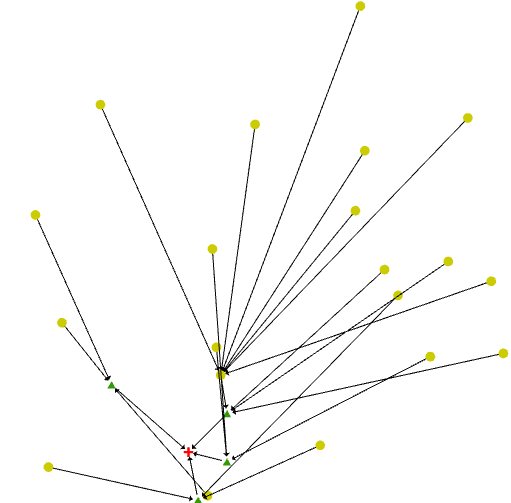
\includegraphics[width=0.8\textwidth]{Chap7/figures/khas_sim}
	\caption{Simulation Example in RePast Simulator}
	\label{fig:sim}
	\end{figure}

Before implementing, we designed the agents required based on the nodes described in the ontology we proposed in Chapter \ref{chap:ont}. Using that, we created a hierarchy of nodes inheriting common properties from a node object. As previously mentioned, we had metrics on range and transmission times from previous experiments and the deployment of LORIS. We used these to create properties for each transmission medium that could be used by each node object. Table \ref{sim:tab:terms} shows how the K-HAS terms, introduced in Chapter \ref{chap:arch}, and LORIS terms, detailed in Chapter \ref{chap:imp}, map to the node types described above. The nodes used in our simulations map directly to the ontology.

	\begin{table}[h]
	\centering
	\begin{tabular}{|l|l|l|}
	\hline
	\textbf{Network Type} & \textbf{Original Term} & \textbf{Maps To}          \\
	\hline
	K-HAS                 & DC Node                & Sensing Node + MK         \\
	                      & DP Node                & Routing Node + HK         \\
	                      & DA Node                & Central Node + HK         \\
	LORIS                 & Buckeye                & Sensing Node + NK         \\
	                      & DA and DP              & Routing/Central Node + HK \\
	\hline
	\end{tabular}
	\caption{Mapping of K-HAS to Simulation Terminology}
	\label{sim:tab:terms}
	\end{table}

Using a Java library we developed for DwC archives during the implementation of LORIS (Section \ref{loris:arch}), we were able to implement DwC archives as the data standard in our simulations, this allowed us to model the prioritisation of sensed data, as well as the classification of observations, in the same way that a K-HAS deployment would.

\section{Network Setup}\label{sim:setup}

\subsection{Parameters}
The parameters used in these simulations were either gained through experiments performed at Danau Girang, gleaned from the data or extracted from technical specifications. Repast allows these parameters to be set in a configuration file and can be manipulated once loaded into the simulation. An example of this file can be seen in Appendix \ref{appendix:sims:params}. The table below outlines the parameters we have used and some that require further explanation are covered in this section.
	\begin{landscape}
	\begin{table} 
	\begin{tabularx}{\textwidth}{|p{4cm}|p{10cm}|p{3cm}|p{2cm}|p{2cm}|}
\toprule
	\textbf{Parameter}                      & \textbf{Description}                                                                                                        & \textbf{Value(s)}   & \textbf{Constant?} & \textbf{Observed?} \\
\midrule
	Sensing Node Count                      & The number of sensing nodes in the network                                                                                  & 20                  & Yes                & No                 \\
	Routing Node Count                      & The number of routing nodes in the network                                                                                  & 4                   & Yes                & No                 \\
	Central Node Count                      & The number of central nodes in the network                                                                                  & 1                   & Yes                & No                 \\
	Height                                  & The height of the available space                                                                                           & 1200                & Yes                & No                 \\
	Width                                   & The width of the available space                                                                                            & 1200                & Yes                & No                 \\
	Capture Chance                          & The chance of an observation being captured each second in normal circumstances                                             & 0.000857703189      & Yes                & No                 \\
	Interesting Chance                      & The chance of an observation containing an item of interest                                                                 & 0.207               & Yes                & No                 \\
	Transmission Rate                       & The transmission rate of sensing nodes in the network                                                                       & Ideal or Variable   & Yes                & No                 \\
	Sensing Node Transmission Rate (Zigbee) & When \textit{Transmission Rate} is set to \textit{ideal}, this is set as the maximum. \textit{Variable} sets this randomly between 20 and the maximum & 20-250 kbps         & No                 & No                 \\
	Sensing Node Transmission Range (Zigbee)& The transmission range of Zigbee                                                                                            & 30                  & Yes                & No                 \\
	Routing Node Transmission Rate (Wi-Fi)  & Always set as the maximum due to the proximity to the central node                                                          & 54000 kbps          & Yes                & No                 \\
	Routing Node Transmission Range (Wi-Fi) & The transmission range of Wi-Fi                                                                                             & 200                 & Yes                & No                 \\
	Bandwidth                               & Determines the available bandwidth in the network, if `saturated' then the chance of capture is increased ten fold          & Normal or Saturated & Yes                & No                 \\
	HK Processing Time                      & Time to process an observation with high knowledge processing capabilities (Central Node or Routing/Sensing Node)           & 30 or 43            & Yes                & No                 \\
	MK Processing Time                      & Time to process an observation with minimal knowledge processing capabilities                                               & 5                   & Yes                & No                 \\
	Observation Size                        & Size of the generated observation, the combination of 3 randomly generated image sizes                                      & 1362-2598 KB        & No                 & No                 \\
	Transmission Time                       & The time an image takes to pass through the network, from point of capture to being received by the central node            & -                   & No                 & Yes      \\
	\bottomrule         
	\end{tabularx}
	\caption{Parameters Used to Configure Repast Simulations}
	\end{table}
    \label{sim:tab:params}
	\end{landscape}

	\subsubsection{Transmission Rate}
	Each scenario, listed in Section \ref{sim:scen}, can be run with either a \textit{variable} or \textit{ideal} transmission rate. This means that the transmission rate of a sensing node can be fixed at the maximum rate at the start of each run or a randomly generated number (between 20 and the maximum) is set at the start of each run. The maximum value was taken from the Zigbee technical specifications.

	%REF

	\subsubsection{Bandwidth, Capture Chance and Interesting Chance}
	As with transmission rate, each scenario can be run with the bandwidth under \textit{normal} or \textit{saturated} load. When the bandwidth is normal, the chance of capture is the value shown in Table \ref{sim:tab:params}, but saturated increases that chance ten fold. A random number is generated on the sensing node every second and compared with the capture chance, generating an observation if the value is less than the chance. 

	Using the existing data collected from Danau Girang, we calculated how often a camera triggers in a six month deployment, as well as how often the observation contained interesting content. 
	
	To calculate the count of interesting images, we processed every directory of images to extract the largest object in the foreground, using our Triton program. Once processed, we iterated through every directory, counted the total number of images and the total number of extracted images; an extracted image is a black and white image containing the largest object that has been found in the observation and are only created when the processing believes that the observation is interesting. This gave us a 20.7\% chance of an image being interesting, across every camera.
	
	The chance of a camera being triggered each second was calculated by the total number of observations (13,399) divided by the number of seconds in six months (15,552,000). This gives a chance of 0.000861561 of a camera trigger in any given second.

	\subsubsection{Transmission Range}
	From our experiments at Danau Girang, see Section \ref{tech:wireless}, we tested the range of Wi-Fi and Zigbee in a humid rainforest, using those values we set trhe transmission range as the maximum that we achieved during our experiments.

	\subsubsection{Observation Size}
	Using the observations we extracted from Danau Girang, we listed the size of all 120,000 files and extracted the minimum and maximum size from the set, when an observation is generated in RePast, it consists of three images and each image is a randomly generated size between the maximum and minimum bounds outlined in the table.

	\subsubsection{Processing Times}
	While the processing times are fixed, central nodes can perform higher knowledge processing slightly faster and they are able to process up to 4 observations at once, whereas routing and sensing nodes can only process one at a time.
	
	\subsubsection{Run Count and Duration}
	Each scenario is configured to run for a period of three months, this is solely due to time constraints due the run time of each simulation. Tests showed that three months was a long enough period to model a saturated network and the capture chance is kept at the six month chance because the network would be deployed for six month periods and these runs serve to show a snippet of their deployment, rather than cover the whole period.
	
	Twenty five runs were completed of each scenario, as well as for the possible combinations of transmission rate and bandwidth. For example, a network simulating NK-NK-NK would have 25 runs for \textit{ideal} transmission rate and \textit{normal} saturation, 25 for \textit{ideal} transmission rate and \textit{saturated} bandwidth and so on.

\subsection{Routing Protocol}
The routing protocol used needs to be dynamic in order to adapt to nodes being added and removed during deployment, while minimising traffic in a resource constrained network. In our approach, we use a modification of the Minimum Cost Forwarding Algorithm (MCFA), described in Section \ref{arch:routing}. A cost is assigned to each node, based on how far they are from the central node, with neighbouring nodes choosing to connect to the node with the lowest cost. However, in normal implementations of MCFA, all nodes are of the same type and simply need to connect to a central node. This protocol is used in all scenarios.

In our K-HAS architecture, sensing nodes cannot connect directly to a central node because processing would not take place. Because of this, we used the same routing method across all scenarios. Our implementation of MCFA works with a discovery phase and a transmission phase. The discovery phase is a scheduled event, taking place at the start of deployment but it can be run throughout deployment to react to nodes being added or removed. 

\subsubsection{Discovery}\label{sim:disc}
	Discovery begins at each central node, scanning nodes in range for routing nodes and sending a broadcast packet, with a cost of 0, to inform them that they are within range of a central node. Links between Central and Routing nodes use W-Fi in all of our scenarios. Once received, routing nodes increment the count and forward the packet to any routing nodes within range of them, where we use the range of Zigbee. We found that this method overloaded the routing nodes and all sensing nodes within range would connect to the first routing node they receive the broadcast from. We then implemented a method, called \textit{load balancing} \cite{Gupta2003}, which uses the sensing nodes connected to a routing node to calculate whether it should offload new nodes to a neighbouring routing node.
	
	The maximum connections a routing node can have is determined by the total number of sensing nodes in the network divided by the total number of routing nodes, which is held in the knowledge base of the central node. Once a routing node has the maximum number of connections allowed, it starts to offload to a neighbouring routing node that is also in range of the sensing node requesting a connection. If there are no neighbouring nodes then the routing node exceeds the maximum number of connections allowed, to save sensing nodes being left with nowhere to send their data.
	
	If the sensing node that receives the broadcast does not have an existing route to a central node, or the cost of the current route is higher than the received route, it adds an edge to the routing node, increments the count and forwards it to all nodes in range. This process continues until the broadcast reaches the edge of the network. Nodes do not have global knowledge of the route to the central node, only of their neighbour with the lowest cost. This can be seen in Figure \ref{fig:dc:discovery} in Section \ref{arch:routing}.
	
	This phase can be repeated throughout the course of the deployment, simply by scheduling it as an event to occur every \textit{n} ticks. However, the simulation currently only uses the discovery phase at the beginning of the deployment.
	
\subsubsection{Transmission}
	Once the discovery phase has been completed, providing nodes are within range of the central node, the transmission phase begins where only DwC archives are then sent across the network. Observations are captured based on the mode of the simulation and sent to the lowest cost neighbour.
	
	In order to manage transmissions, nodes have a \textit{SendState} object that contains the next archive to send, the time it will take to send it and whether it is currently sending. This is used to determine what operations to perform. Once an archive has been sent, it is deleted from the SendState and the sending flag is set to false. A new archive is then added and sent when the opportunity arises.
	
	When a routing node receives the archive, it begins processing. Routing nodes use the SendState as well, but they only add an archive once it has been processed and they then select the oldest archive that has been classified as interesting, providing an archive is not already waiting to be sent. The archive stores information about the route it takes, recording every hop, as well as the time it took from capture to central node.
	
	Scheduled sending events run every thousand ticks, which is configurable, to check the sending state of the node and send any archives in the SendState. The node then waits for the number of ticks that it will take in order to transmit the archive.
	
	Once the simulation is completed, either manually or through a defined number of ticks, the archives in each node are iterated over and written to a CSV file, with details such as the path it took, total transmission time and time of capture.


\subsection{Observation Transmission}
When a node has no knowledge, it simply sends the observation that was first added to its queue. With MK, it finds the first \textit{interesting} observation and sends that, if one is not in the queue then an observation marked as \textit{unknown}. HK performs much the same as MK except it instead looks for \textit{empty} observation if an \textit{interesting} cannot be found. If a node has any form of knowledge processing power, it will not send an observation unless it has first been processed. Nodes can only send an observation one at a time and must also wait for the receiving node to be free.

An observation is marked as delivered once it has been received by the central node, if there is only processing at the central node, then delivery is delayed until the central node has processed it.

\subsection{Processing}
Repast has built in functionality that allows for methods to be scheduled to start at a certain tick and repeat at set intervals. The way a scheduled method works is that it is run at the time specified and further scheduled methods can be prevented from running until it has completed. Much of the node's functionality is handled in this way. A processing method is set to run every 10 ticks (seconds) to replicate the functionality of checking a file system for new observations. The earliest (unprocessed)observation is found and a processing method is scheduled, depending on the knowledge level of the node. The function for DA nodes is the same, except they are able to process 4 observations simultaneously. This is shown in listing \ref{alg:sim:proc} and listing \ref{alg:sim:know} shows how classifications are made. 

Observations are passed to the processing methods and those methods run for the specified durations. High knowledge processing nodes are able to determine an empty observation with 97\% accuracy and detect an object of interest with 82\% accuracy. A random number is generated and compared with these values, to determine how the observation is classified. Once the observation has been classified, the node marks itself as not processing to allow a new observation to be classified. 

\begin{lstlisting}[breaklines=true, caption={Processing Function for DA and DP Nodes}, label={alg:sim:proc}, language=java]
kL = getKnowledgeLevel()
if(kL == NoKnowledge OR isProcessing) {
	return
}else{
	obs = getEarliestObservation()
	if(obs.identification IS NULL OR (obs.identification NOT NULL AND obs.identifiedBy.getKnowledgeLevel() < kL)) {
		if (kL == MinimalKnowledge) {
			schedule method for minimal processing to run as soon as possible for 5 ticks
			setProcessing(true)
		}else if(kL == HighKnowledge) {
			schedule method for high processing to run as soon as possible for 43 ticks
			setProcessing(true)
		}
	}
}
\end{lstlisting}
\vfill
\begin{lstlisting}[breaklines=true, caption={Processing Functions for Nodes}, label={alg:sim:know}, language=java]
void highKnowledge(obs) {
	rand = generateRandomNumber()
	interestingAccuracy = 0.82
	emptyAccuracy = 0.97
	if(obs.actualContent = "INTERESTING") {
		if R < interestingAccuracy
			obs.id = "INTERESTING"
		else
			obs.id = "UNKNOWN"
	}else{
		if R < emptyAccuracy
			obs.id = "EMPTY"
		else
			obs.id = "UNKNOWN"
	}
	if(this == centralNode)
		obs.processingTime += 30
	else
		obs.processingTime += 43
	setProcessing(false)
}
void lowKnowledge(obs) {
	rand = generateRandomNumber()
	interestingAccuracy = 0.1
	if(obs.actualContent = "INTERESTING") {
		if R < interestingAccuracy
			obs.id = "INTERESTING"
		else
			obs.id = "UNKNOWN"
	}else{
		obs.id = "UNKNOWN"
	}
	obs.processingTime += 5
	setProcessing(false)
}

\end{lstlisting}

\section{Results}\label{sim:res}
% \subsection{In-Network Processing}
In this section, we show plots for each scenario and the variations on bandwidth and transmission rate. The resulting CSV files from each run were processed with the R programming language \cite{rlang} and summary statistics were output to find the mean transmission time for all observations, interesting and empty, as well as those that were delivered to the end point during the runtime of the simulation.

 Table \ref{tab:delnum} shows the number of observations delivered for each scenario and their variations. We can see that almost all observations are delivered when the network is not saturated and the transmission rate is ideal, despite Zigbee's low transmission rate. As knowledge is pushed out into the network, the processing time becomes a factor on top of the transmission time and we can see that this reduces the number of received observations. MK-HK-NK is the lowest here and we believe that is because it is the only scenario that processes an observation twice (with MK and then HK), but we discuss this in greater detail as we analyse the results further. As we discussed previously, processing on the DA node means that an observation is only marked as delivered when it has been processed. However, the short processing times (when compared to long transmission times) and the fact that a DA node can process up to four observations in parallel means that this is not really a bottleneck.
 
\begin{landscape}
\begin{table}[htbp]
    \begin{tabular}{rrrrrrr}

    \toprule
    Mode  & Bandwidth & Transmission Rate & All   & Delivered & Undelivered & \% Delivered \\
    \midrule
    % NK-NK-NK & normal & ideal & 44524.6 & 44501 & 24    & 100 \\
    % NK-NK-NK & normal & variable & 44437.6 & 30088 & 14350 & 68 \\
    % NK-NK-NK & saturated & ideal & 444955.2 & 89933 & 355022 & 20 \\
    % NK-NK-NK & saturated & variable & 444858.9 & 48830 & 396029 & 11 \\
\rowcolor{Gray}    
    NK-NK-MK & normal & ideal & 44408 & 44255 & 153   & 100 \\
\rowcolor{Gray}
    NK-NK-MK & normal & variable & 44538.8 & 35131 & 9407  & 79 \\
\rowcolor{Gray}
    NK-NK-MK & saturated & ideal & 444714 & 129224 & 315490 & 29 \\
\rowcolor{Gray}
    NK-NK-MK & saturated & variable & 444569.6 & 66454 & 378115 & 15 \\
    NK-NK-HK & normal & ideal & 44480.73 & 44478 & 3     & 100 \\
    NK-NK-HK & normal & variable & 44512.4 & 32804 & 11708 & 74 \\
    NK-NK-HK & saturated & ideal & 444898.5 & 134552 & 310347 & 30 \\
    NK-NK-HK & saturated & variable & 444759.8 & 57105 & 387655 & 13 \\
\rowcolor{Gray}
    NK-MK-NK & normal & ideal & 44500.93 & 40614 & 3887  & 91 \\
\rowcolor{Gray}
    NK-MK-NK & normal & variable & 44429.87 & 27981 & 16448 & 63 \\
\rowcolor{Gray}
    NK-MK-NK & saturated & ideal & 444858.2 & 106656 & 338202 & 24 \\
\rowcolor{Gray}
    NK-NK-NK & saturated & variable & 444649.5 & 50643 & 394006 & 11 \\
    MK-NK-NK & normal & ideal & 44483.8 & 44206 & 278   & 99 \\
    MK-NK-NK & normal & variable & 44533.13 & 26307 & 18226 & 59 \\
    MK-NK-NK & saturated & ideal & 444593.7 & 92904 & 351690 & 21 \\
    MK-NK-NK & saturated & variable & 444988.9 & 51225 & 393764 & 12 \\
\rowcolor{Gray}
    MK-HK-NK & normal & ideal & 44513.73 & 40927 & 3586  & 92 \\
\rowcolor{Gray}
    MK-HK-NK & normal & variable & 44455.47 & 23638 & 20817 & 53 \\
\rowcolor{Gray}
    MK-HK-NK & saturated & ideal & 443211.3 & 79864 & 363347 & 18 \\
\rowcolor{Gray}
    MK-NK-NK & saturated & variable & 444397.5 & 46454 & 397943 & 10 \\
    HK-NK-NK & normal & ideal & 44423.73 & 43378 & 1045  & 98 \\
    HK-NK-NK & normal & variable & 44437.33 & 29295 & 15142 & 66 \\
    HK-NK-NK & saturated & ideal & 445257 & 97790 & 347467 & 22 \\
    HK-NK-NK & saturated & variable & 444816.9 & 46061 & 398756 & 10 \\
    \bottomrule

    \end{tabular}%
    \caption{All Observations Captured and Delivered}
\end{table}%
\label{tab:delnum}%
\end{landscape}

%%%NormIdeal
\subsection{Normal Network}

When the network is not saturated and Zigbee is able to transmit observations at its maximum transmission rate, we can see that the transmission rate increases the further we push knowledge out into the network (Figure \ref{fig:sim:res:norm:ideal:delmean}). However, higher knowledge at the edge of the network significantly reduces the transmission time for an interesting observation. MK-HK-NK is higher than even MK-MK-MK because of its increased processing time, although MK-HK-NK is able to more accurately determine TPs.

Figure \ref{fig:sim:res:norm:ideal:delundel} shows that all scenarios delivered the majority of the observations captured. MK-HK-NK delivered around 95\% but this is likely due to the processing time discussed previously. The reduced number for NK-MK-NK is odd, we believe it is because the DP nodes become a bottleneck for processing as they can only process a single observation at a time. Because the network was not saturated, the delivered observations are consistent with the configuration parameters outlined in Table \ref{sim:tab:params}.

With a variable transmission rate, nodes could transmit anywhere from 20kbps to the maximum 250kbps that Zigbee provides, Figure \ref{fig:sim:res:norm:variable:delundel} shows how this affects the number of delivered observations. Central processing allows for the greatest number of observations to be delivered and we expected that NK-NK-NK would deliver almost everything. We are unsure as to why this is.

\begin{figure}

\begin{subfigure}{\textwidth}
\centering
  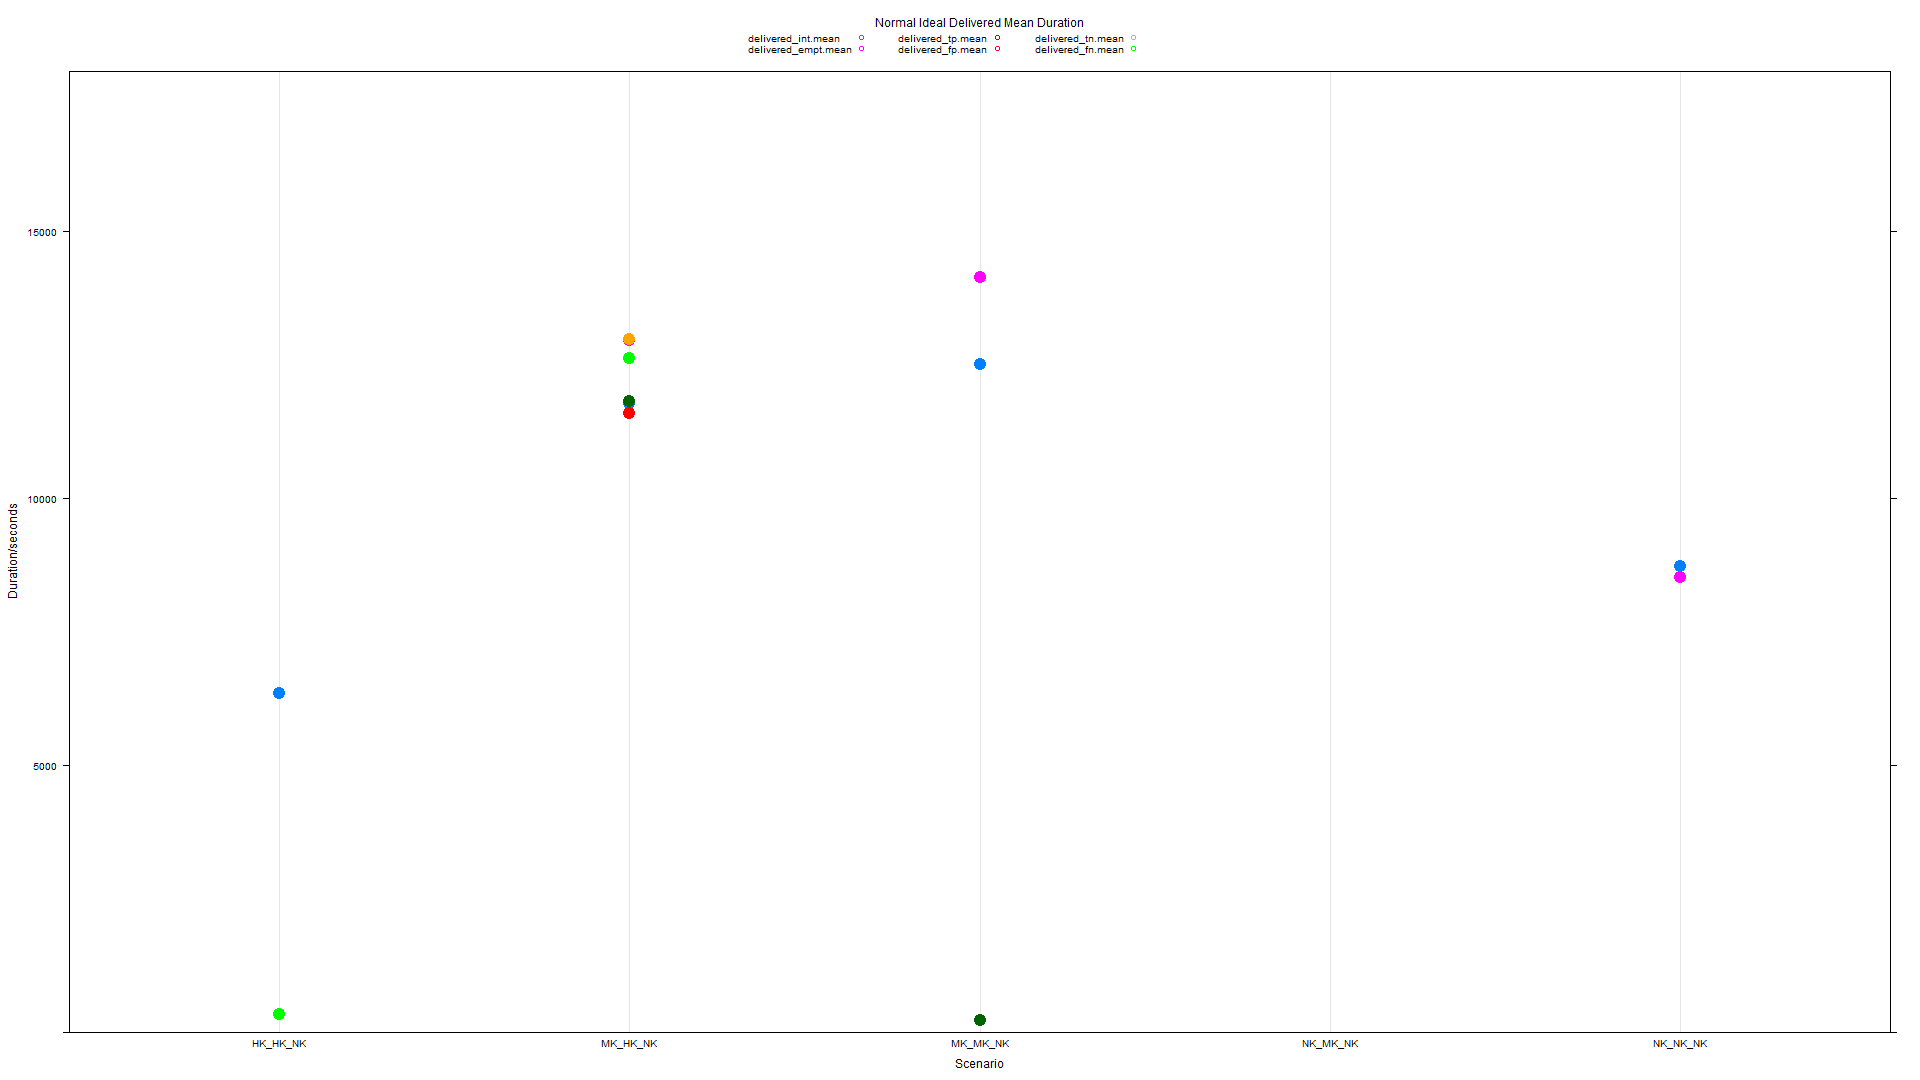
\includegraphics[height=.5\textheight]{Chap7/figures/plots/normal_ideal/delivered_mean.png}
  \caption{Ideal Transmission Rate}
\label{fig:sim:res:norm:ideal:delmean}
\end{subfigure}%
\vfill
\begin{subfigure}{\textwidth}
\centering
  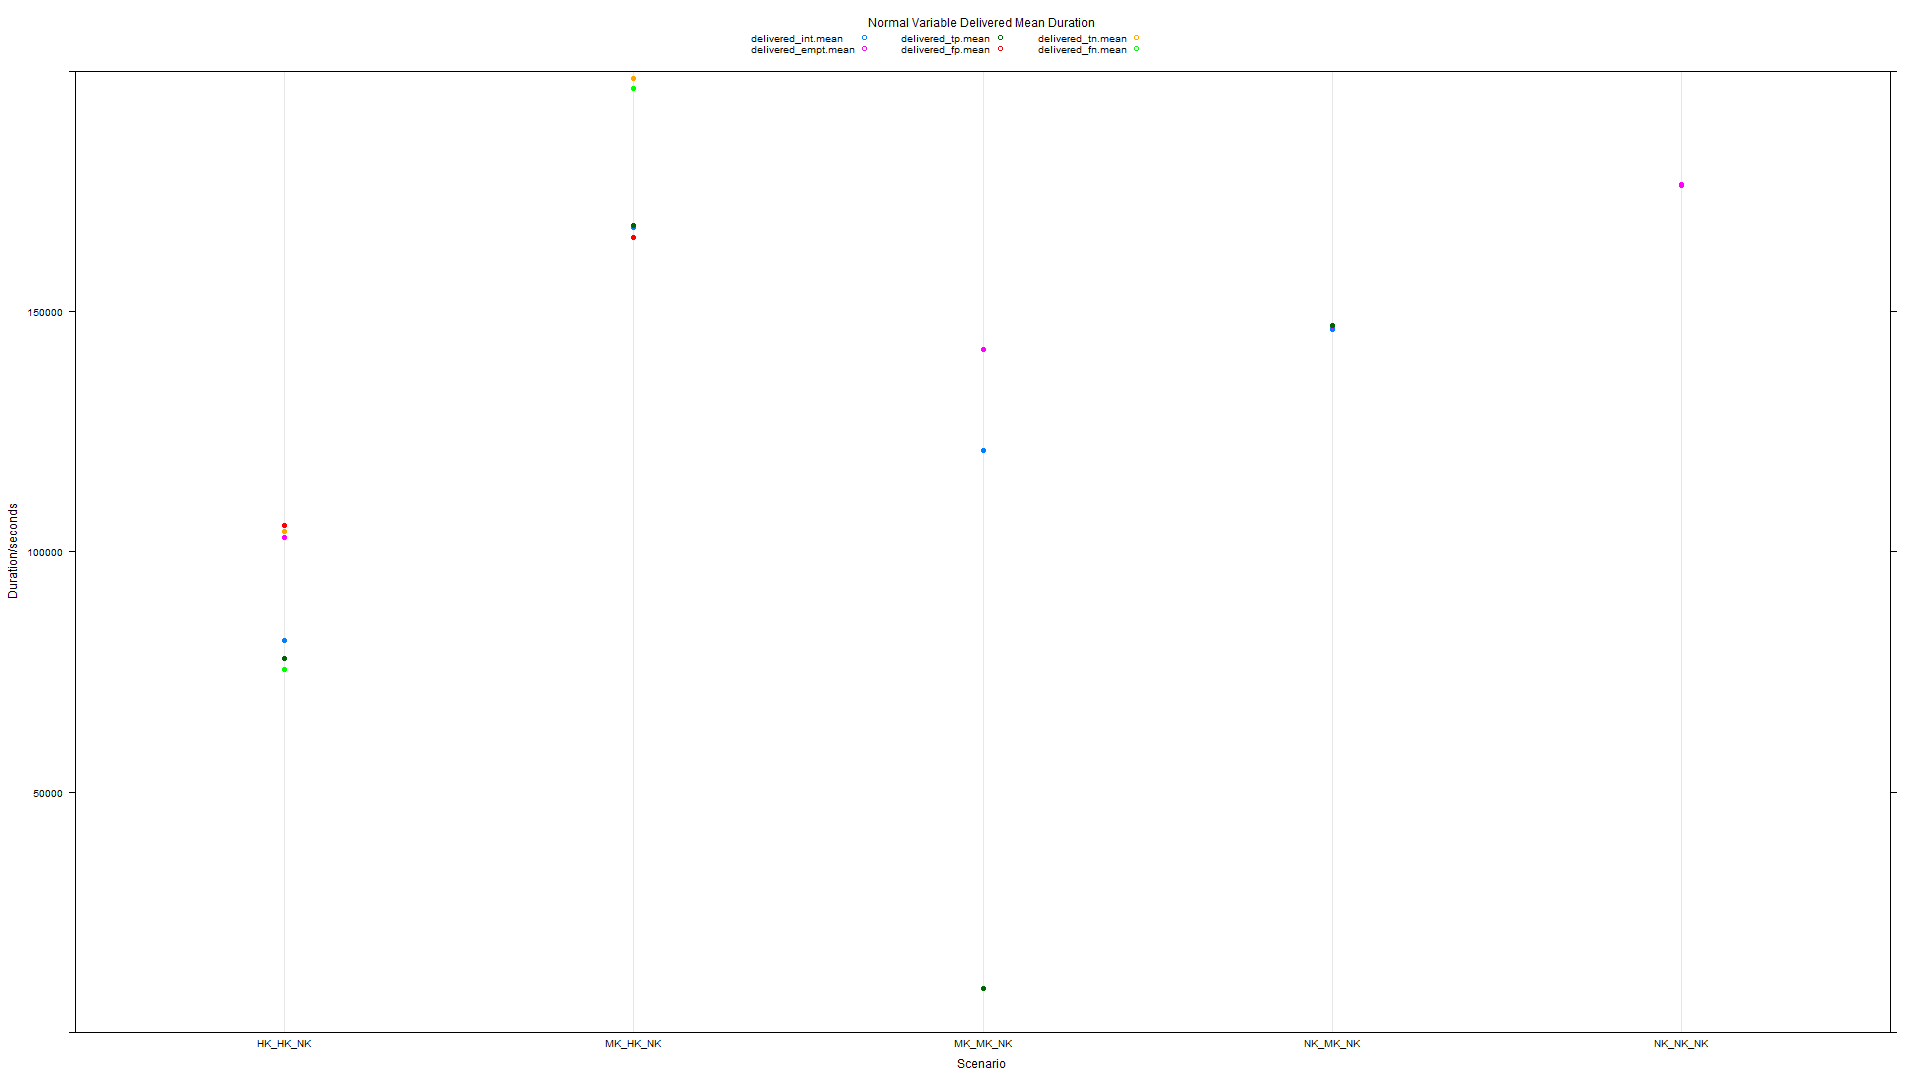
\includegraphics[height=.5\textheight]{Chap7/figures/plots/normal_variable/delivered_mean.png}
  \caption{variable Transmission Rate}
	\label{fig:sim:res:norm:variable:delmean}
\end{subfigure}
\caption{Mean Transmission Times for Delivered Observations for a Normal Network}
\end{figure}

\begin{figure}[H]
\centering
\begin{subfigure}{.5\textwidth}
  \centering
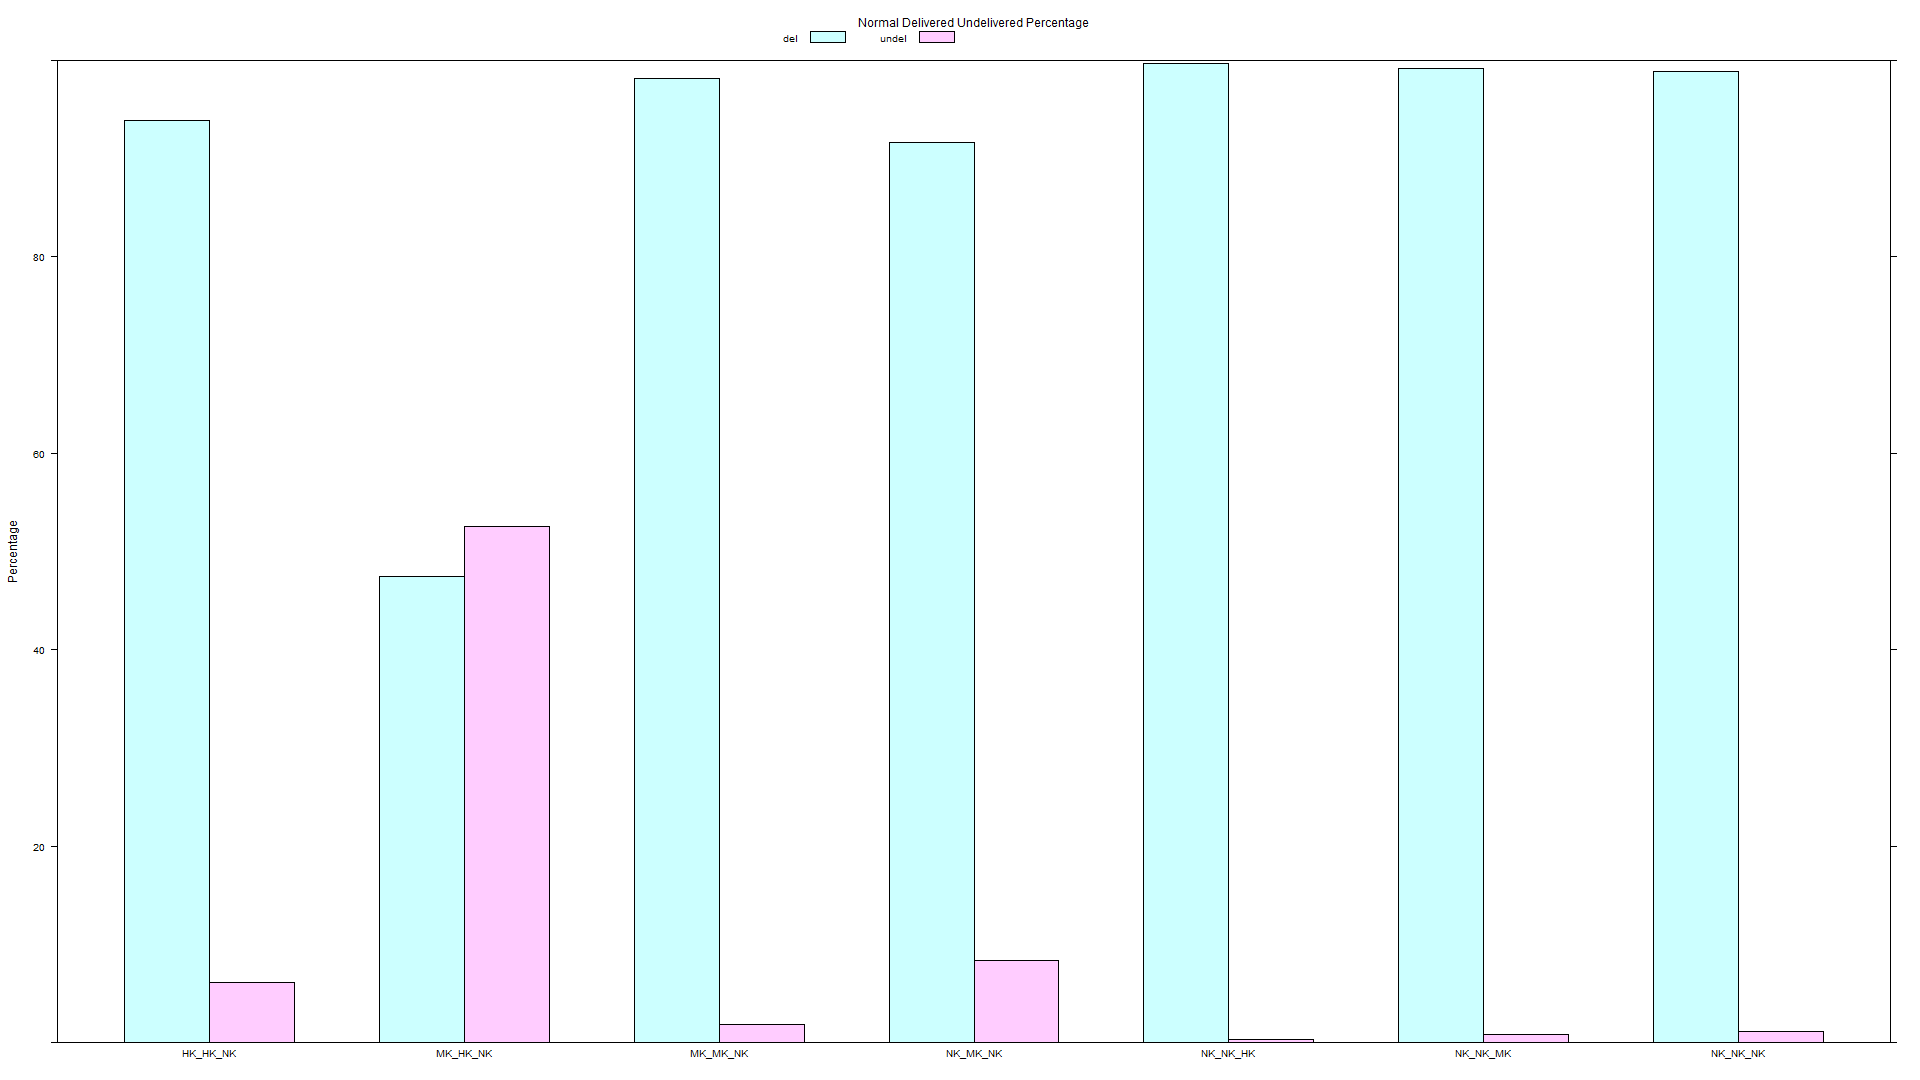
\includegraphics[width=\linewidth]{Chap7/figures/plots/normal_ideal/delvsundel_percent.png}
  \caption{Ideal Transmission Rate}
\label{fig:sim:res:norm:ideal:delundel}
\end{subfigure}%
\begin{subfigure}{.5\textwidth}
  \centering
	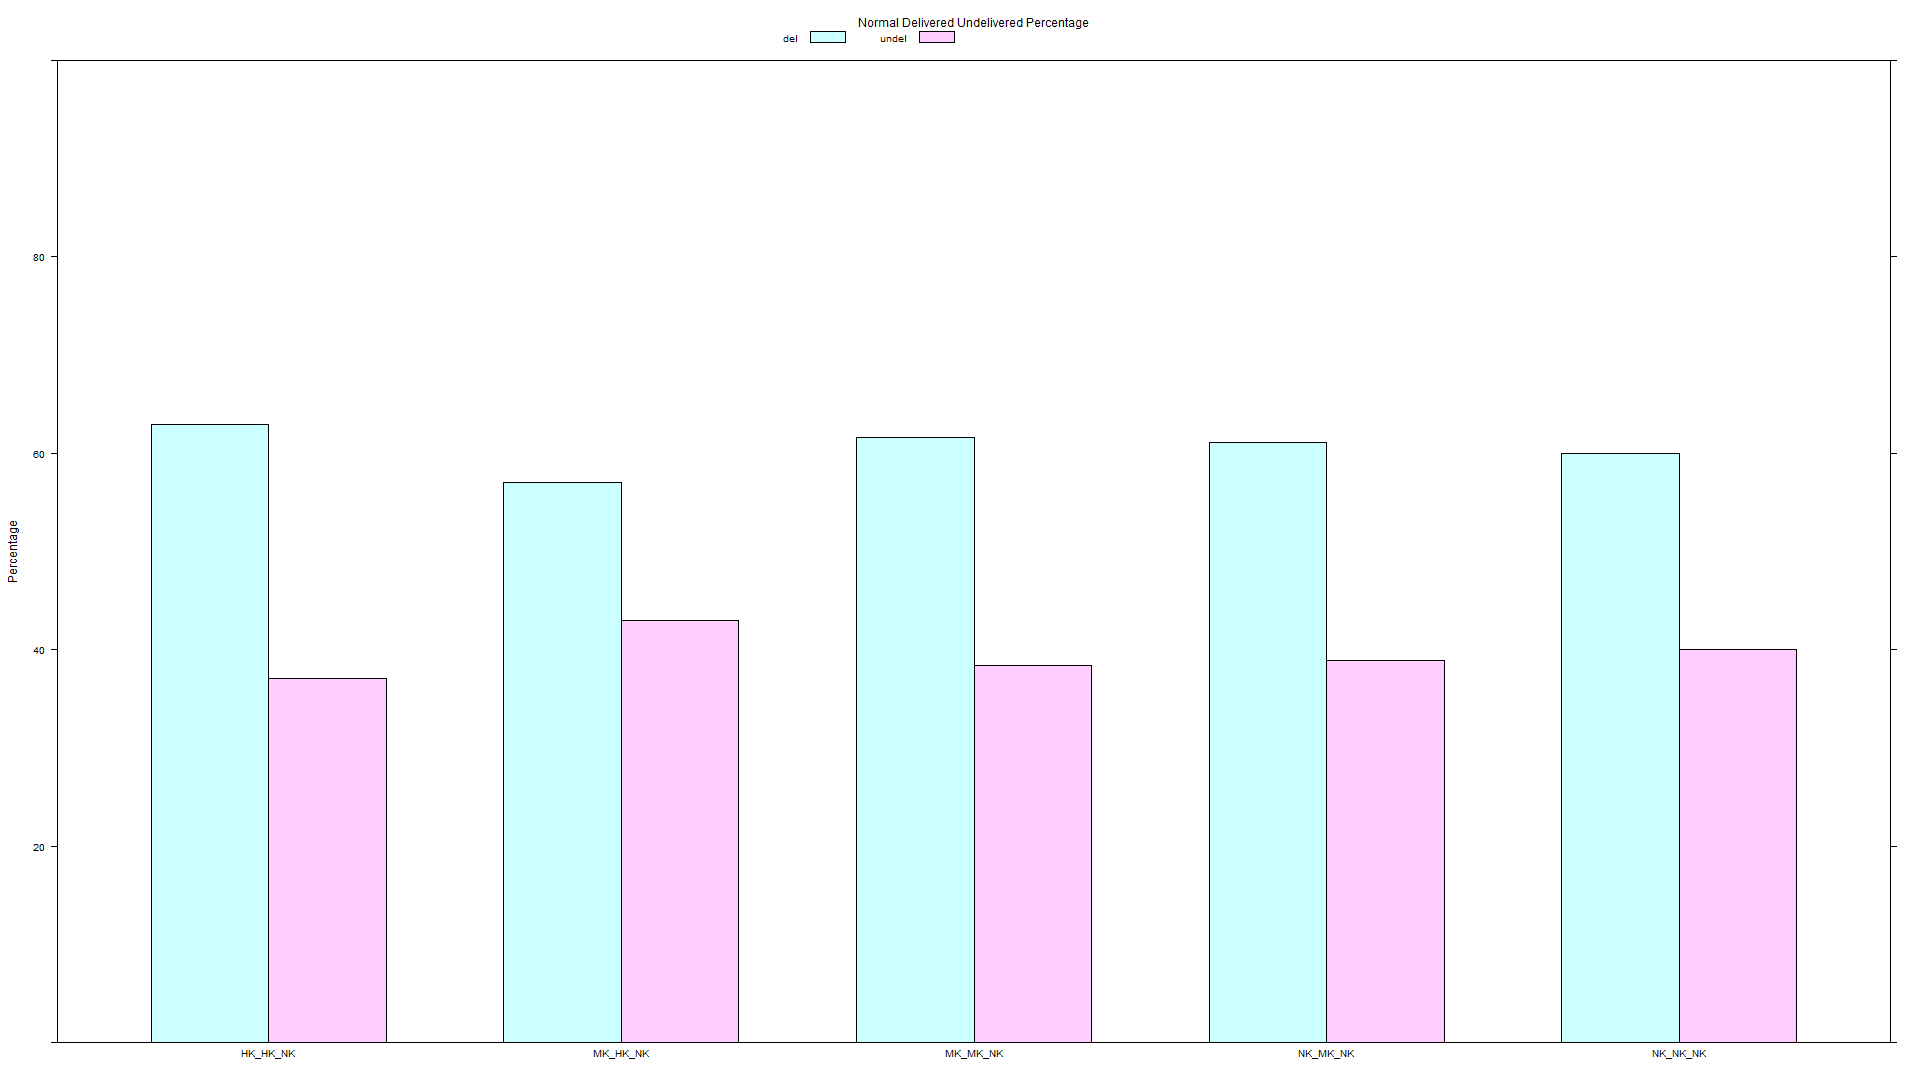
\includegraphics[width=\linewidth]{Chap7/figures/plots/normal_variable/delvsundel_percent.png}
  \caption{variable Transmission Rate}
	\label{fig:sim:res:norm:variable:delundel}
\end{subfigure}
\caption{Delivered vs Undelivered Observations for a Normal Network}
\end{figure}

\begin{figure}[H]
\centering
\begin{subfigure}{.5\textwidth}
  \centering
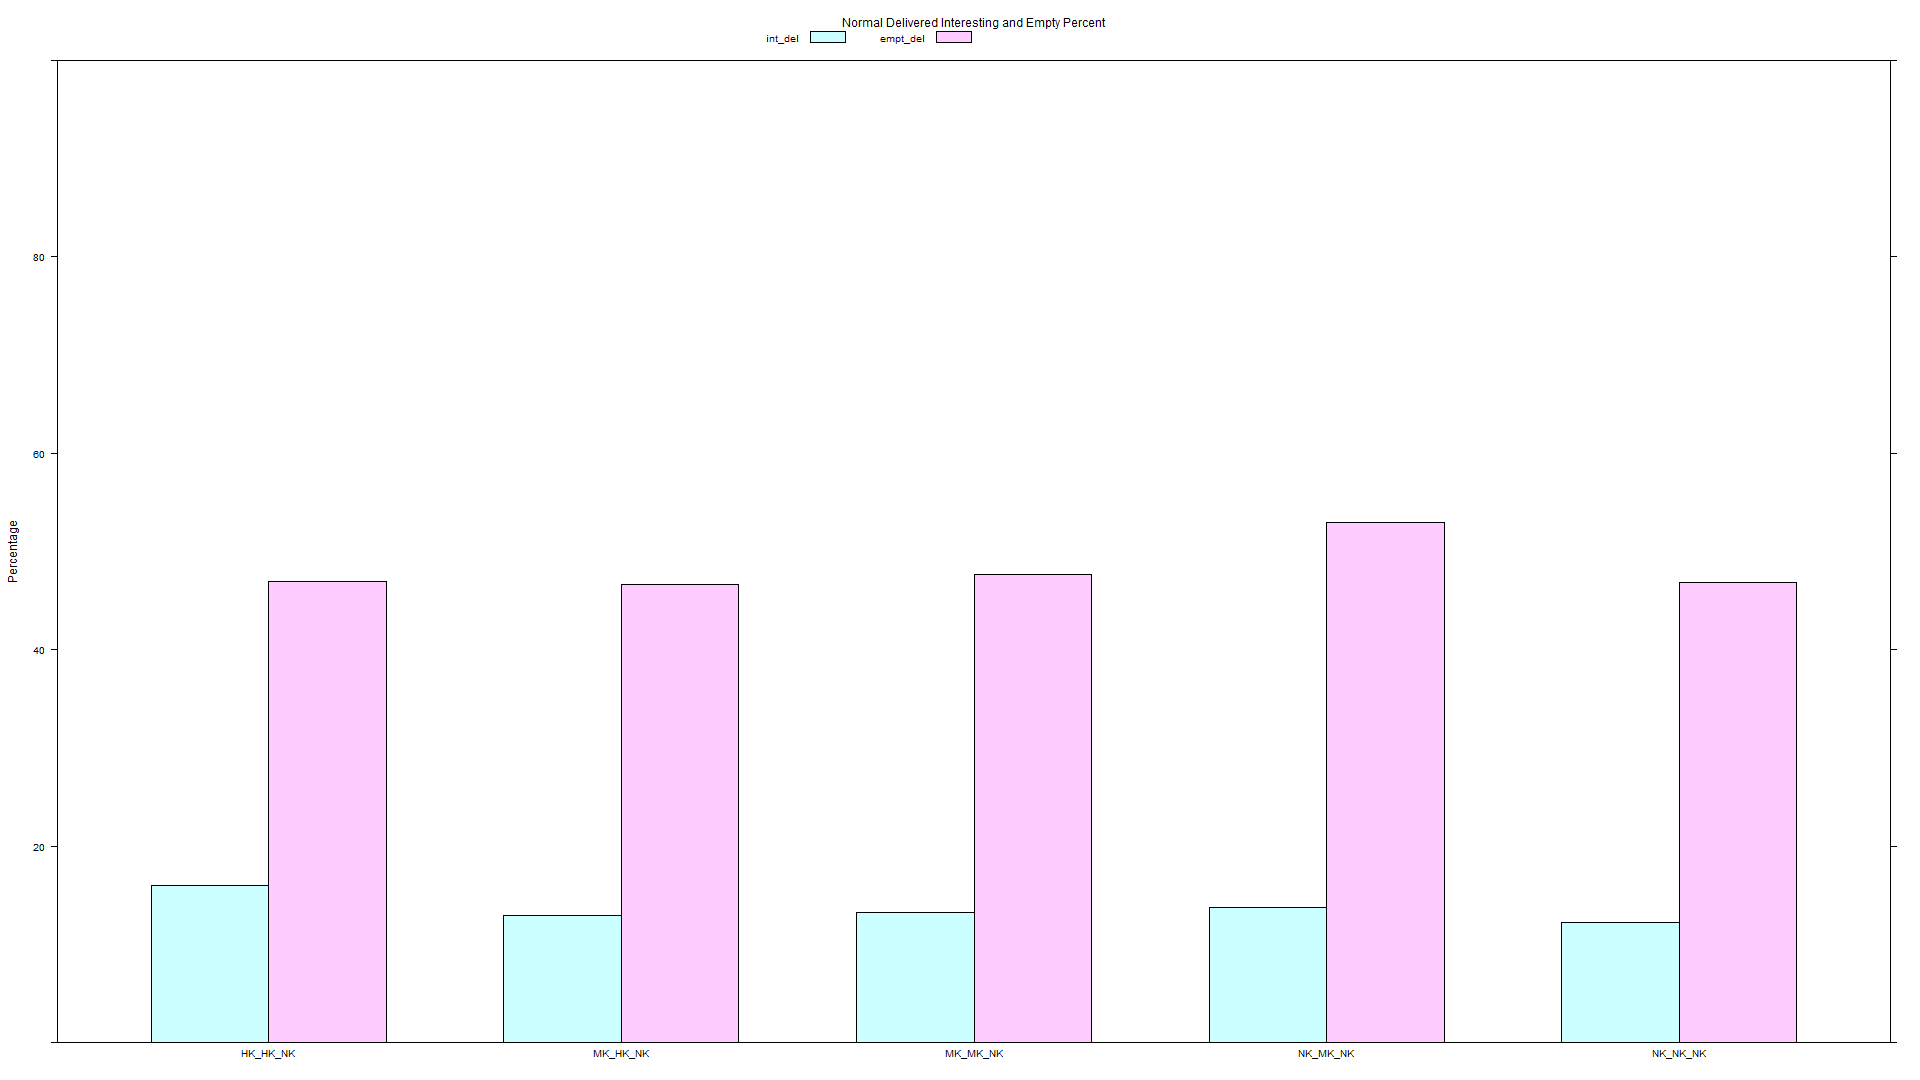
\includegraphics[width=\textwidth]{Chap7/figures/plots/normal_variable/emptvsint_percent.png}
  \caption{Ideal Transmission Rate}
	\label{fig:sim:res:norm:ideal:emptint}
\end{subfigure}%
\begin{subfigure}{.5\textwidth}
  \centering
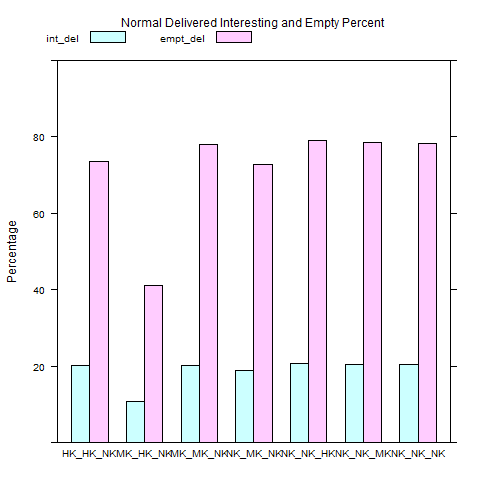
\includegraphics[width=\textwidth]{Chap7/figures/plots/normal_ideal/emptvsint_percent.png}
  \caption{variable Transmission Rate}
	\label{fig:sim:res:norm:variable:emptint}
\end{subfigure}
\caption{Interesting vs Empty Delivered Observations for a Normal Network}
\end{figure}

\subsection{Saturated Network}
The transmission time for both ideal and variable transmission rates is greatly increased when the network is saturated and we expected these scenarios to show how pushing knowledge further into the network provides more interesting observations faster, prioritising when the network is aware that it cannot deliver every observation it has captured.

	The pattern in Figure \ref{fig:sim:res:sat:ideal:delmean} is similar to those of Figures \ref{fig:sim:res:norm:ideal:delmean}and \ref{fig:sim:res:norm:variable:delmean}. Scenarios of central processing (and no knowledge) are consistently high, as is NK-MK-NK because nodes cannot prioritise data from the edge. HK-NK-NK is much faster when delivering interesting observations, which would also reduce the mean transmission time for all observations but we did not expect to see a reduction in the time taken for empty observations when compared with other scenarios. This is most likely because the processing time of HK-NK-NK means that fewer observations are delivered in each run (Figure \ref{fig:sim:res:sat:ideal:delundel}) but could also be because of empty observations misclassified as interesting being prioritised through the network as it is the only scenario that can mark an observation as empty from the edge. However, the higher accuracy of HK-HK-NK should mean that fewer misclassifications are made. 
	
\begin{figure}[H]
\centering
\begin{subfigure}{\textwidth}
  \centering
  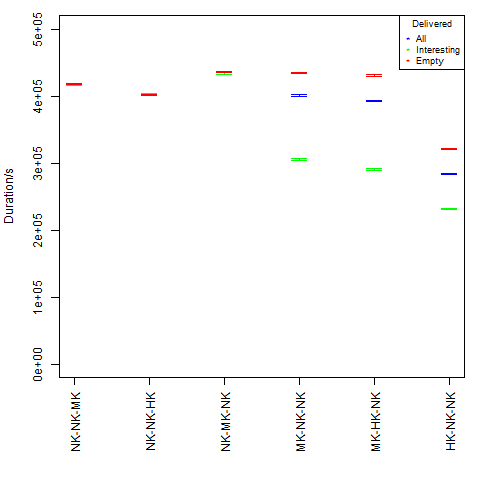
\includegraphics[height=.5\textheight]{Chap7/figures/plots/saturated_ideal/delivered_mean.png}
  \caption{Ideal Transmission Rate}
	\label{fig:sim:res:sat:ideal:delmean}
\end{subfigure}%
\vfill
\begin{subfigure}{\textwidth}
  \centering
  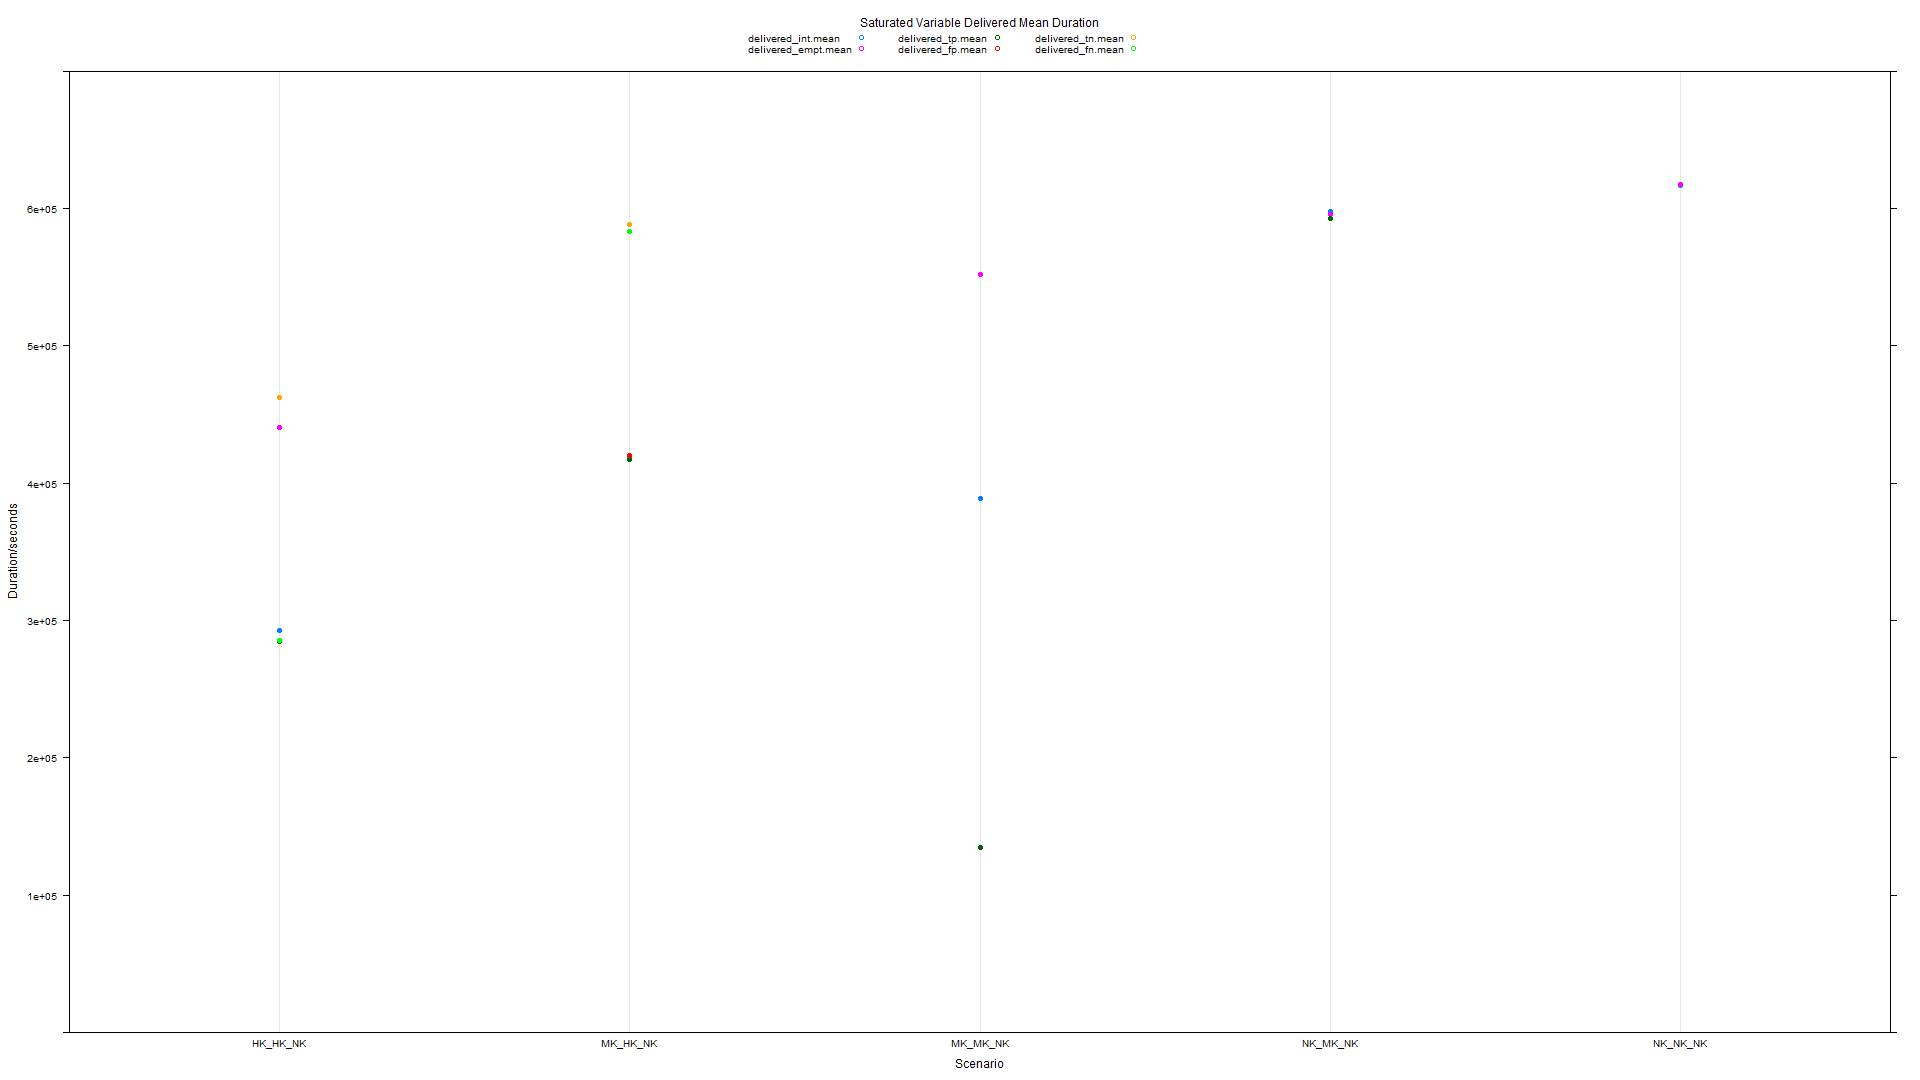
\includegraphics[height=.5\textheight]{Chap7/figures/plots/saturated_variable/delivered_mean.png}
  \caption{variable Transmission Rate}
	\label{fig:sim:res:sat:variable:delmean}
\end{subfigure}
\caption{Mean Transmission Times for Delivered Observations for a Saturated Network}
\end{figure}
	
	\begin{figure}[H]
\centering
\begin{subfigure}{.5\textwidth}
  \centering
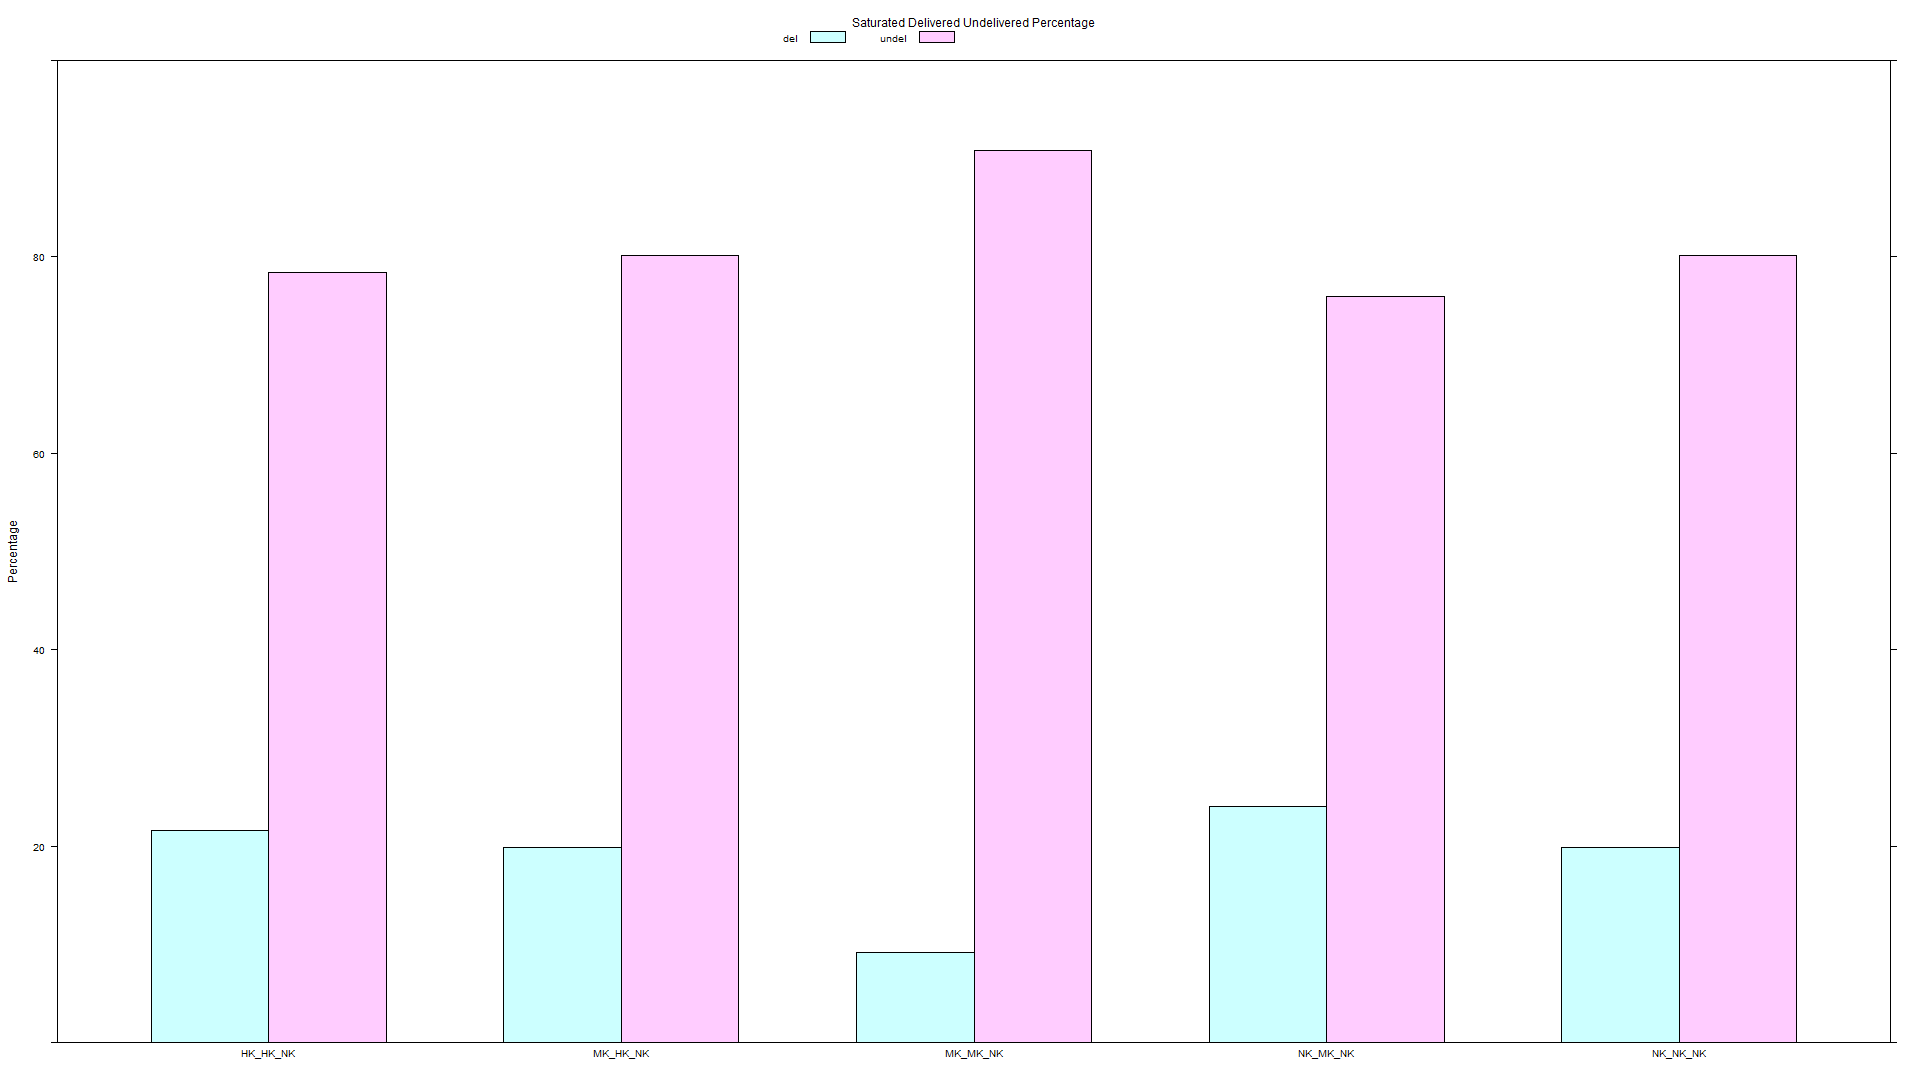
\includegraphics[width=\linewidth]{Chap7/figures/plots/saturated_ideal/delvsundel_percent.png}
  \caption{Ideal Transmission Rate}
\label{fig:sim:res:sat:ideal:delundel}
\end{subfigure}%
\begin{subfigure}{.5\textwidth}
  \centering
	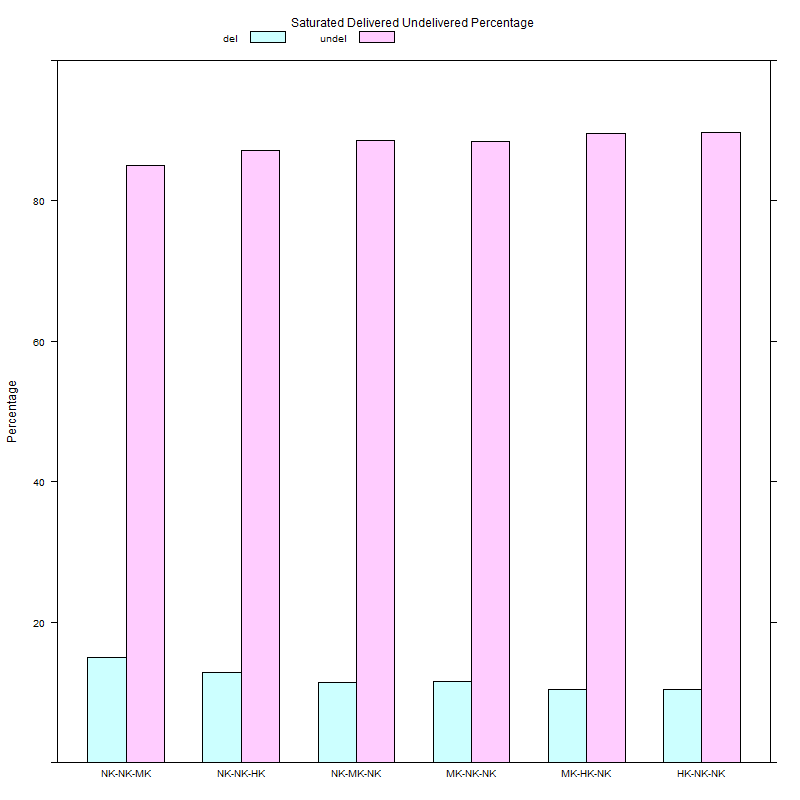
\includegraphics[width=\linewidth]{Chap7/figures/plots/saturated_variable/delvsundel_percent.png}
  \caption{variable Transmission Rate}
	\label{fig:sim:res:sat:variable:delundel}
\end{subfigure}
\caption{Delivered vs Undelivered Observations for a Normal Network}
\end{figure}

\begin{figure}[H]
\centering
\begin{subfigure}{.5\textwidth}
  \centering
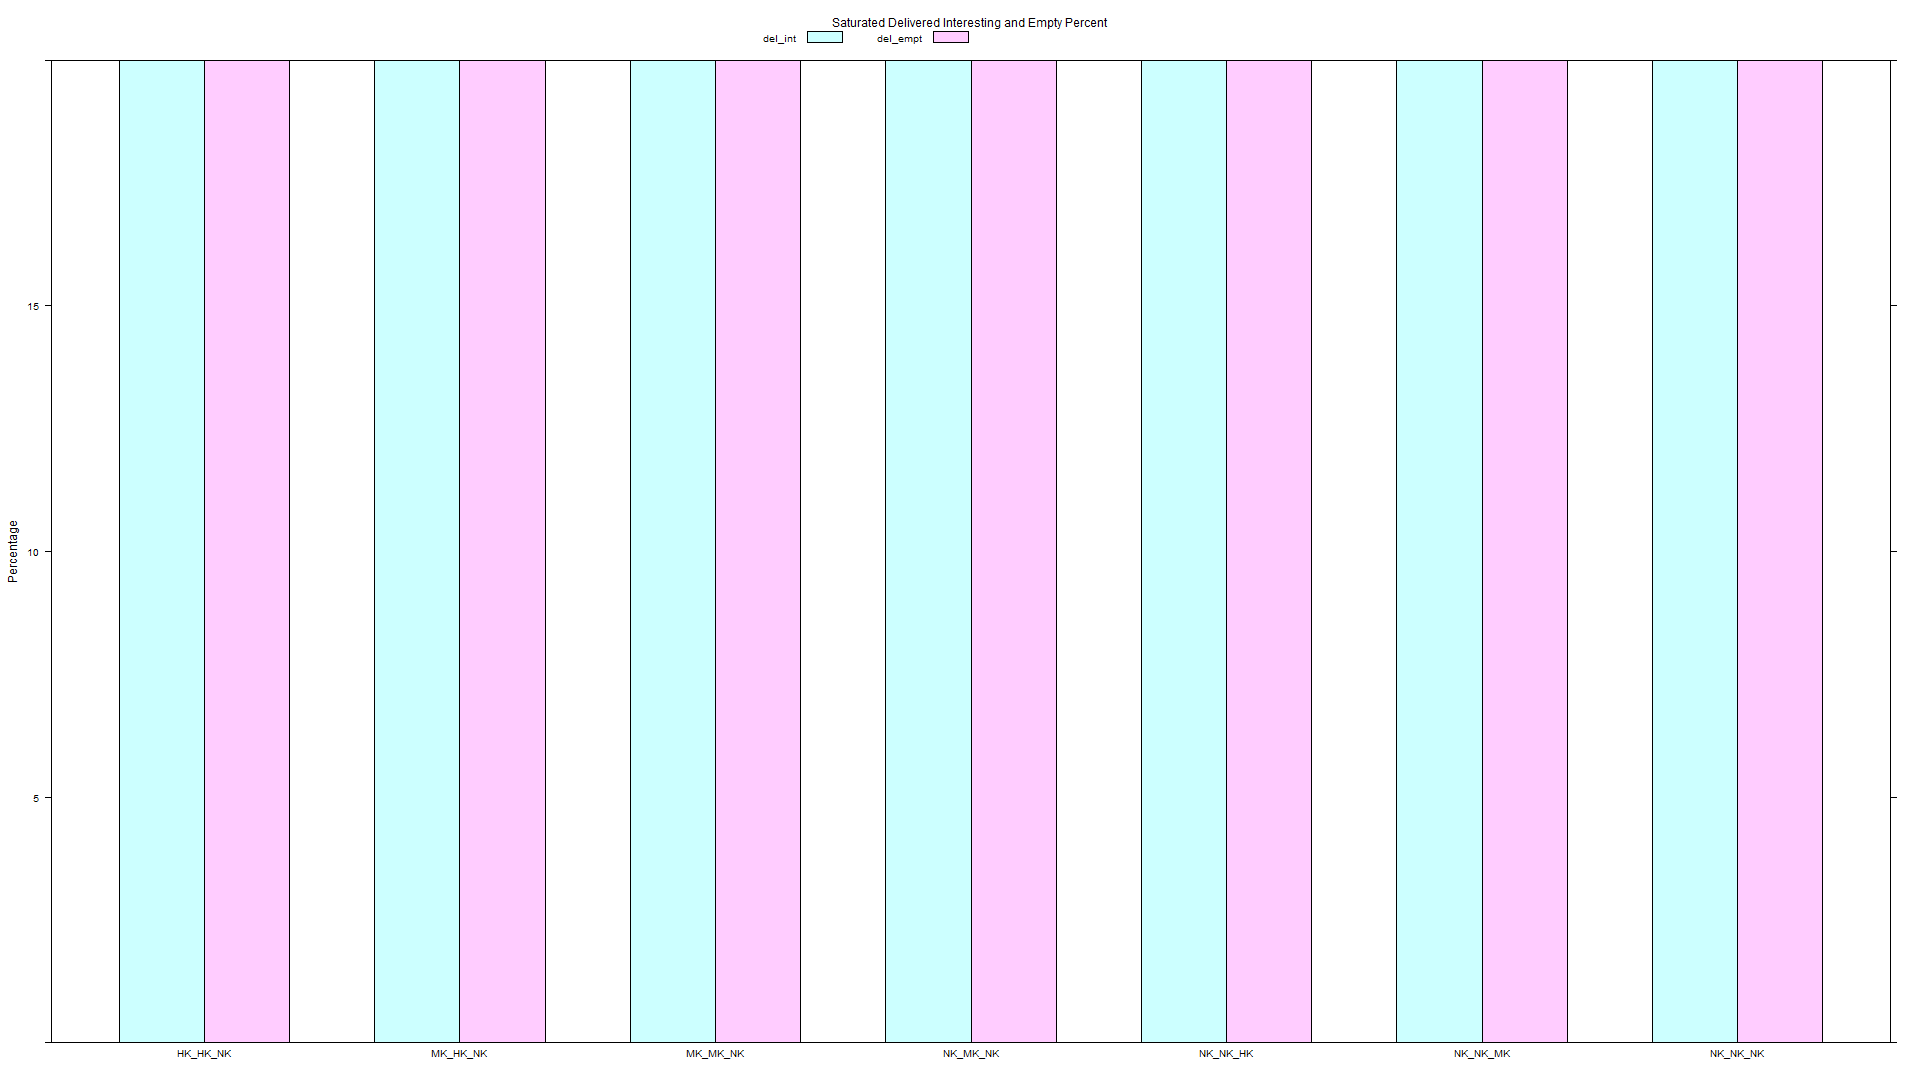
\includegraphics[width=\linewidth]{Chap7/figures/plots/saturated_ideal/emptvsint_percent.png}
  \caption{Ideal Transmission Rate}
	\label{fig:sim:res:sat:ideal:emptint}
\end{subfigure}%
\begin{subfigure}{.5\textwidth}
  \centering
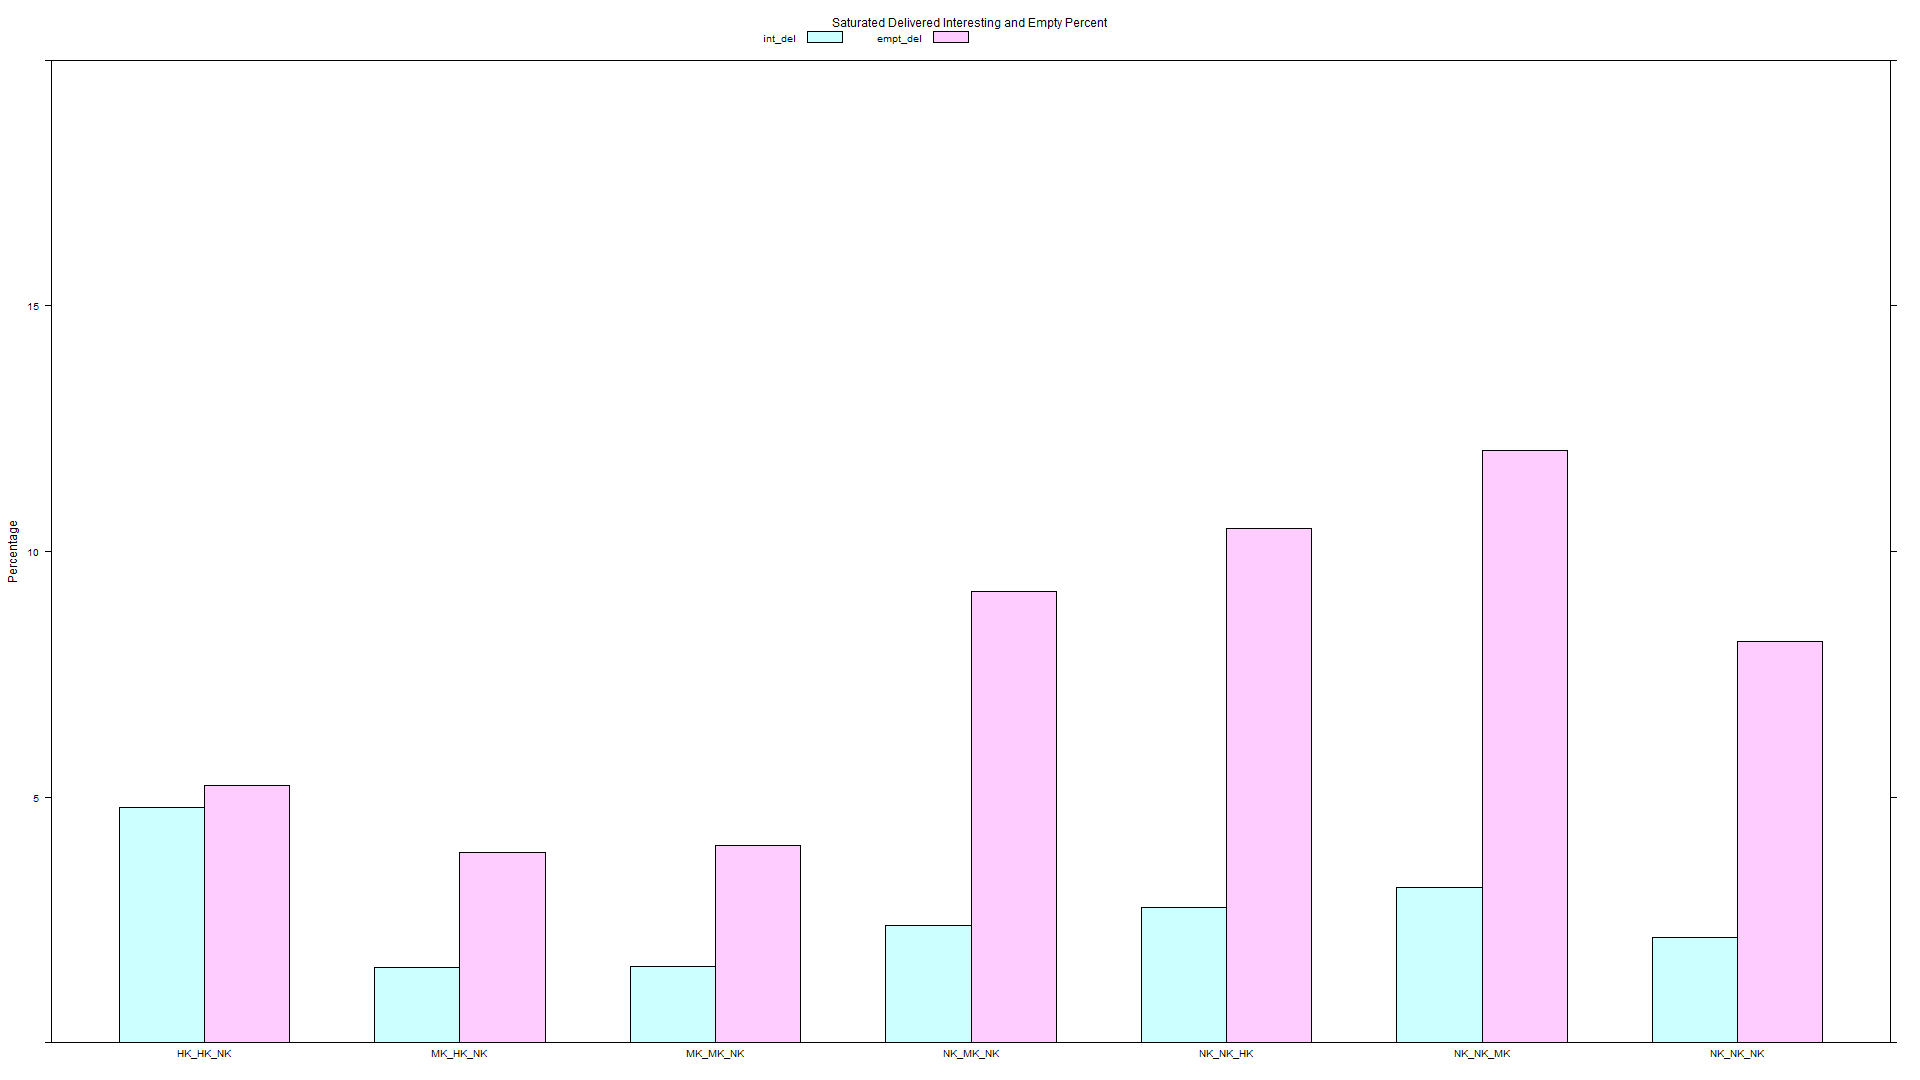
\includegraphics[width=\linewidth]{Chap7/figures/plots/saturated_variable/emptvsint_percent.png}
  \caption{variable Transmission Rate}
	\label{fig:sim:res:sat:variable:emptint}
\end{subfigure}
\caption{Interesting vs Empty Delivered Observations for a Normal Network}
\end{figure}



\section{Conclusion}\label{sim:conc}
The general trend that is clear from all the figures is that pushing knowledge further out into the network increases the transmission time of all observations, when compared to central/no processing, but it does speed up the delivery of interesting observations, especially when the network is saturated.

These simulations first show that saturating the network simply by increasing the chance of capture ten fold can have a huge impact on the transmission time of observations and really tests how each scenario prioritises data within the network. While processing each observation can take time depending on whether the node possesses minimal or high knowledge processing capabilities, it does not seem to be the bottleneck here. With nodes only having a single radio, sending in parallel is not possible and waiting for a neighbouring node to be available can delay an observation massively.

Pushing knowledge further out into the network does reduce the time taken for an interesting observation to reach the central node. When the network is saturated, it is clear to see how the prioritisation can impact what data is delivered and that higher knowledge processing capabilities allows for interesting data to be delivered faster and with a higher priority. The downside to MK-HK-NK is that this processing needs to occur twice: once at the data collection node and again on the data processing node and it seems that this adds a delay to observations. However, in many situations, it may not be possible to put high knowledge processing nodes throughout the network as they are more expensive, more powerful nodes that would likely draw more power.

If the requirement of a sensor network was to deploy a network that had no time restriction on when data was delivered but context was required then central processing is the more logical choice. However, if interesting data needed to be prioritised then using nodes with knowledge at the edge of the network allows for that prioritisation and, while the time to process is an overhead, it does prioritise well enough that the data aggregation becomes a stream of data based on importance, as well as time captured.



% \section{Conclusion} \label{sim:conc}
	
% In this chapter, we have detailed the development of simulations to show the different scenarios for pushing knowledge out to the edge of a network. Using different levels of knowledge processing capabilities on nodes, we have shown that a network with HK processing capabilities can detect and prioritise interesting images, while simultaneously delaying empty images for a time when the network is not busy. However, using a network that solely comprises of HK nodes results in a battery life that lasts for 3 weeks on each node. The MK-HK network architecture we have proposed provides a combination of HK and MK nodes, distributed based on their role in the network. For example, nodes tasked with sensing and forwarding images only have MK processing capabilities. These simulations have shown that the HK-MK scenario results in a delay of interesting image delivery, when compared to MK-ALL, but the percentage of interesting images delivered is significantly increased.

% Using a model of real world transmission rates, we have seen that the variation in transmission times can be quite large, but the difference between MK-HK and HK-ALL is not that great. This suggests that our MK-HK proposal (K-HAS) is the best solution for most scenarios as it provides a longer network lifetime with the same ratio of TP:FN images as a network where every node is equipped with HK.

% While the simulation is not feature complete, it is accurate enough to show how MK-HK utilises the knowledge-processing capabilities at each tier to process, and prioritise, sensed data based on knowledge gained from the environment, previously sensed data and from humans using the network. Our results also show that the difference between MK-HK and HK-ALL is  not significant enough to warrant the loss in network lifetime. However, not every scenario would be suited to this. NK-MK shows a slightly faster transmission time and a much longer network lifetime, as most nodes would not have any processing power. While the processing of sensed data would not be enough to rely on, it could act as pre-processing that could be processed further once power is not an issue. This would be well suited for networks where nodes have limited power and are not easily accessible, such as bird nest monitoring networks. 

% MK-HK allows sensed data to be processed, and delivered, in near real-time with approximately 82\% of all interesting data being correctly classified. This number could increase the longer that the network is deployed, which is something we would like to investigate in the future.

% Finally, we simulated the situation where there is more sensed data than the bandwidth available. The greater knowledge-processing capabilities of HK-ALL scenarios ensured that empty images were delayed and interesting observations were sent with a greater priority. While there were interesting observations misclassified as empty that were delayed, they made up less than 10\% of all interesting observations. MK-HK did receive fewer interesting observations, most likely due to its limited ability to prioritise sensed data right from the edge of the network, but the majority of interesting observations were true positives and they were prioritised over empty observations. MK-ALL, with a longer network lifetime of MK-HK and HK-ALL, did not prioritise interesting over empty data effectively but still provided more true positives than false negatives.

% We can conclude that, for a power efficient WSN, the results from these simulations suggest that MK-HK can deliver many of the same benefits that HK-ALL provides while not pushing HK to the edge of the network, reducing the network lifetime. If power was of no concern, HK-ALL is able to deliver more interesting observations and prioritise more accurately from the edge of the network, as well as filtering important data more effectively when the network is saturated.

% \subsection{Central Processing}

% \subsubsection{Normal Bandwidth and Ideal Transmission Rate}
% 	\begin{figure}[H]
% 	\centering
% 	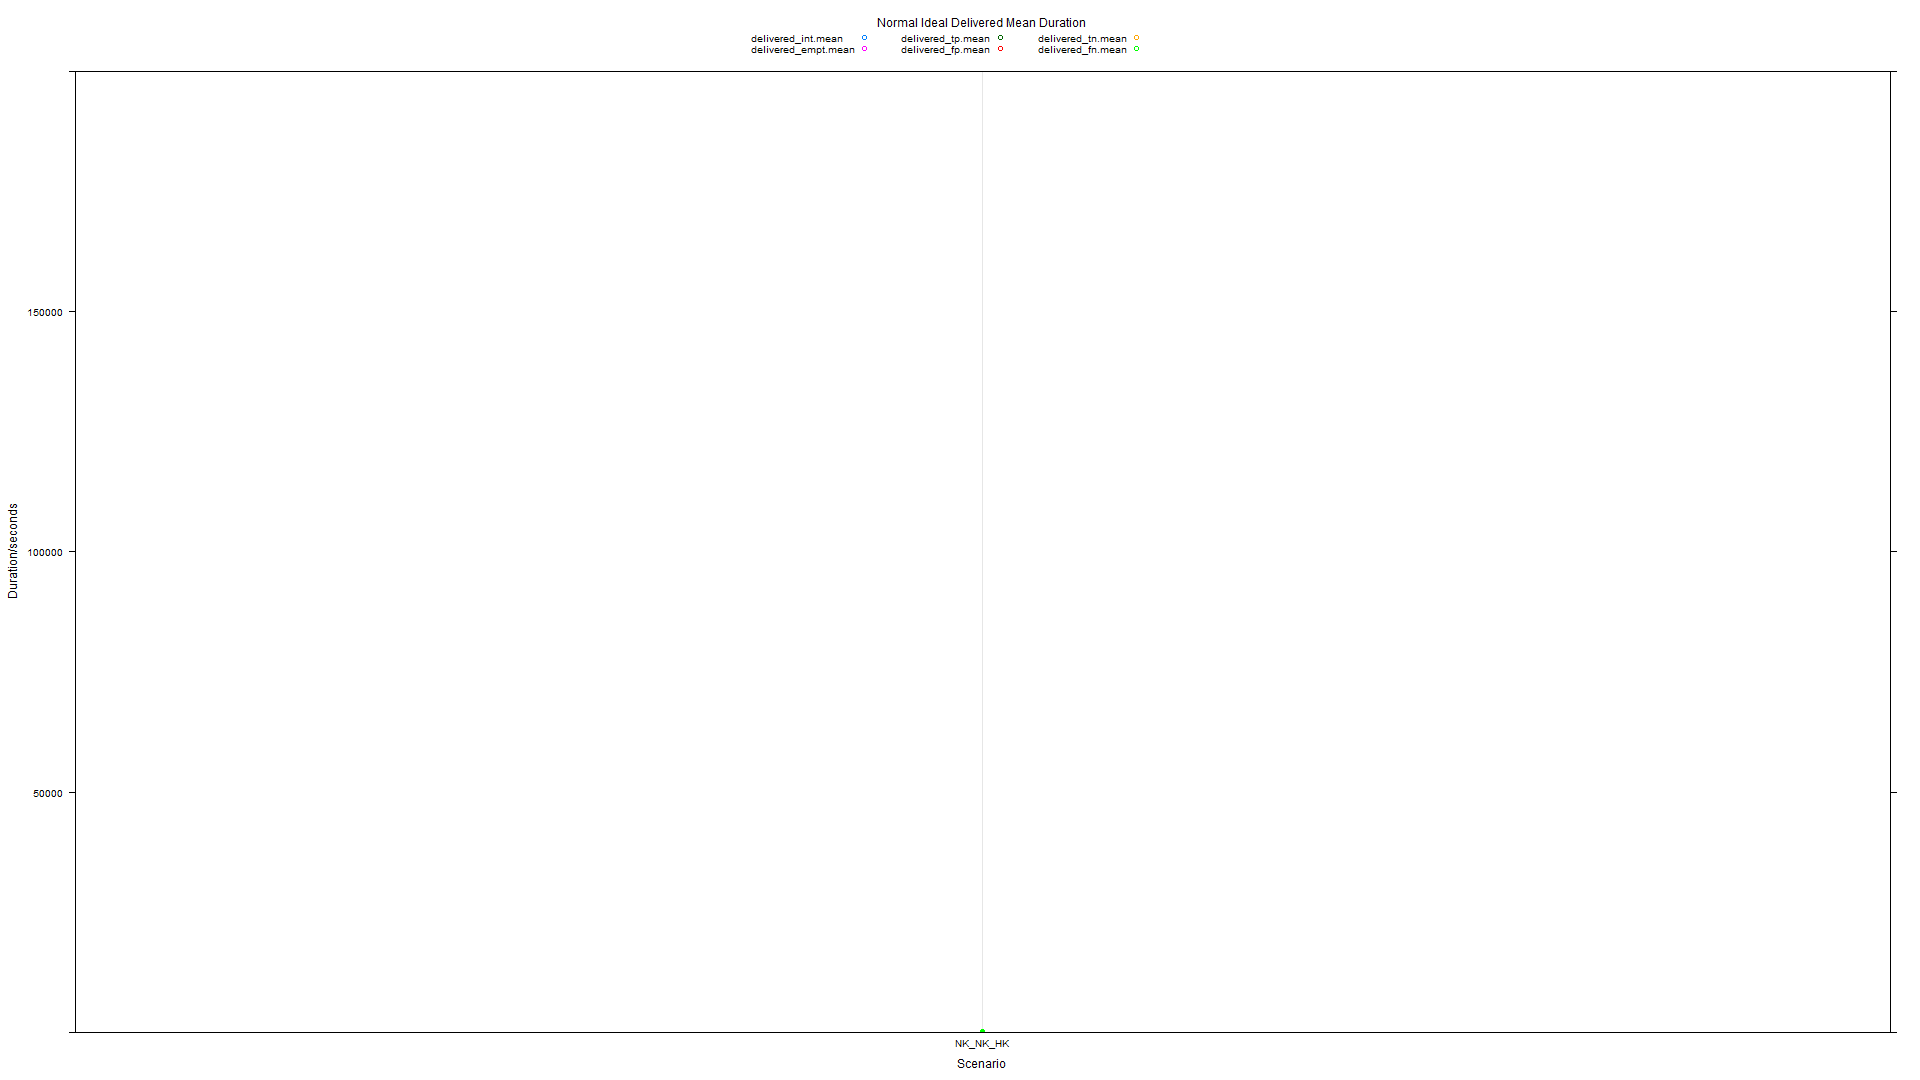
\includegraphics[width=0.8\textwidth]{Chap7/figures/plots/normal_ideal/delivered_mean_central.png}
% 	\caption{Delivered Observations Mean Transmission Time for Normal Saturation and Ideal Transmission Rate}
% 	\label{fig:sim:res:norm:ideal:delmean}
% 	\end{figure}

% 	\begin{figure}[H]
% 	\centering
% 	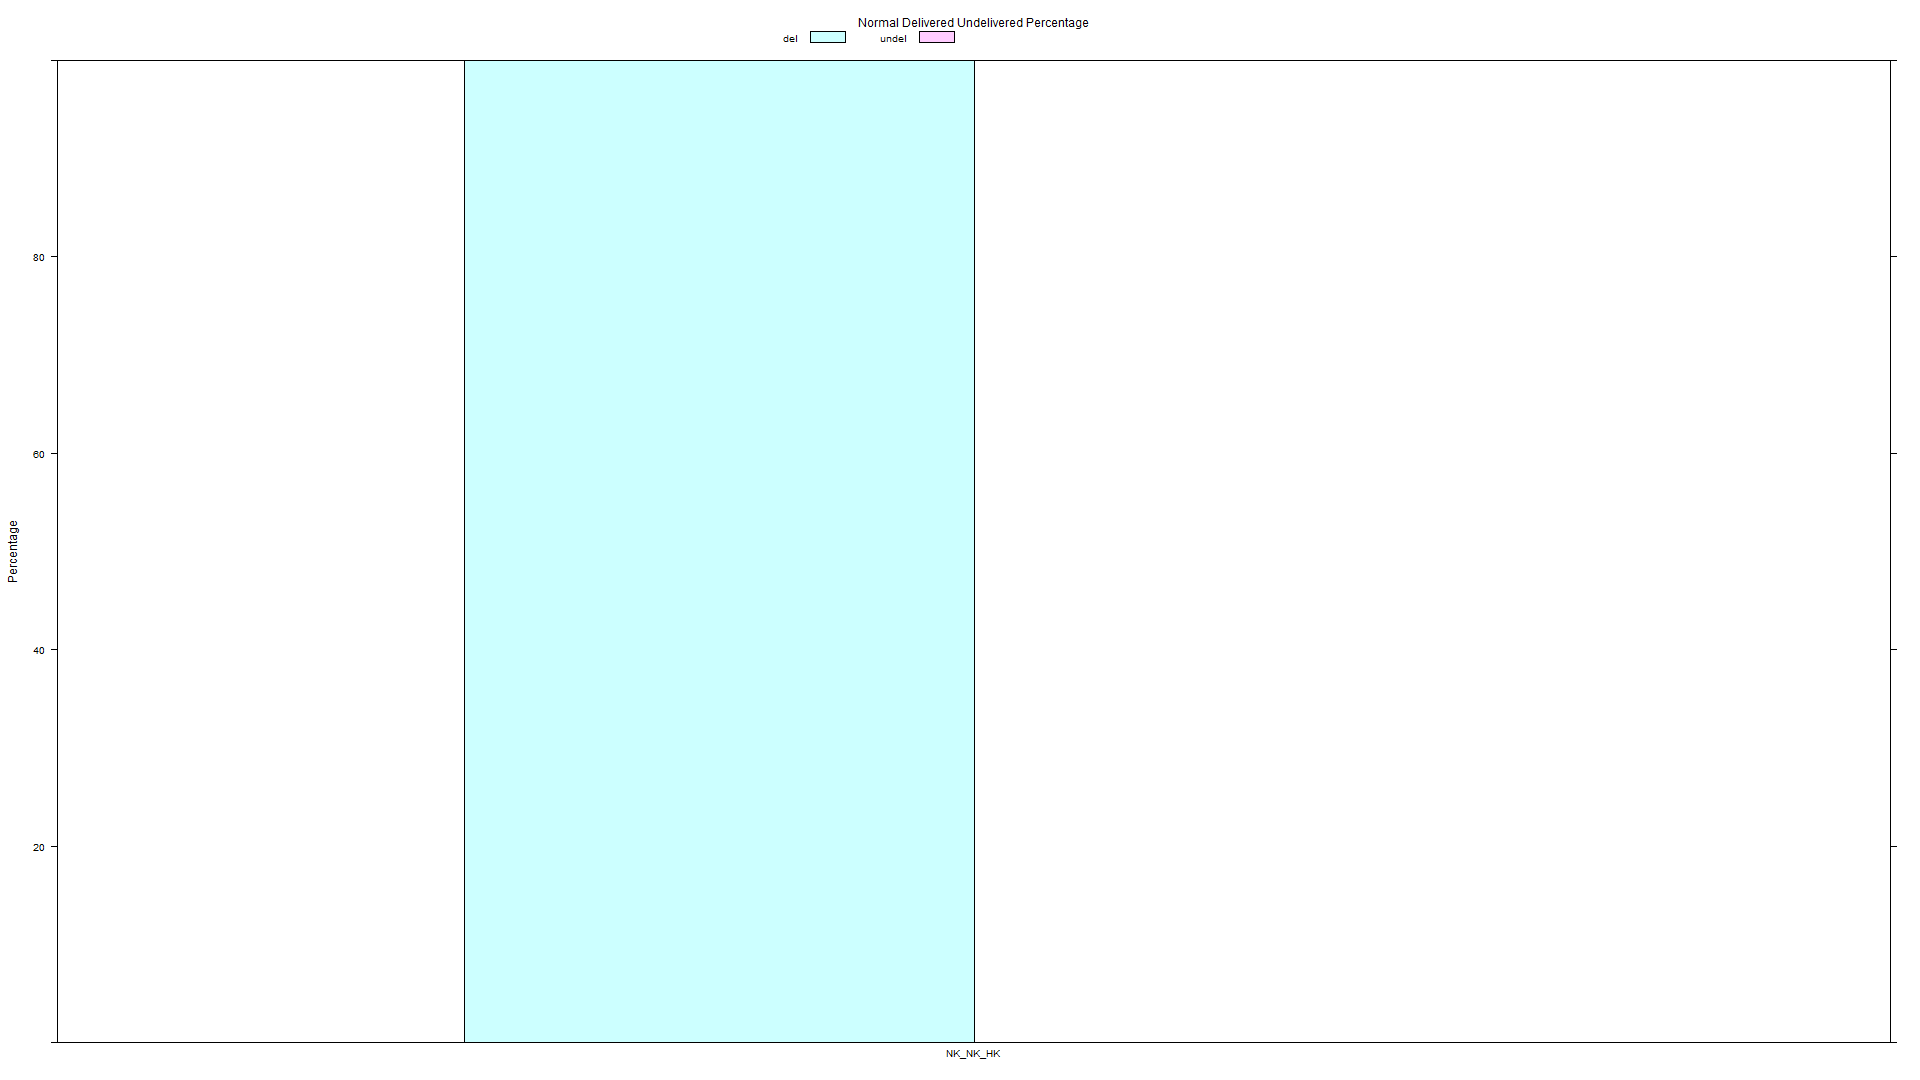
\includegraphics[width=0.8\textwidth]{Chap7/figures/plots/normal_ideal/delvsundel_percent_central.png}
% 	\caption{Delivered vs Undelivered Observations for Normal Saturation and Ideal Transmission Rate}
% 	\label{fig:sim:res:norm:ideal:delundel}
% 	\end{figure}

% 	\begin{figure}[H]
% 	\centering
% 	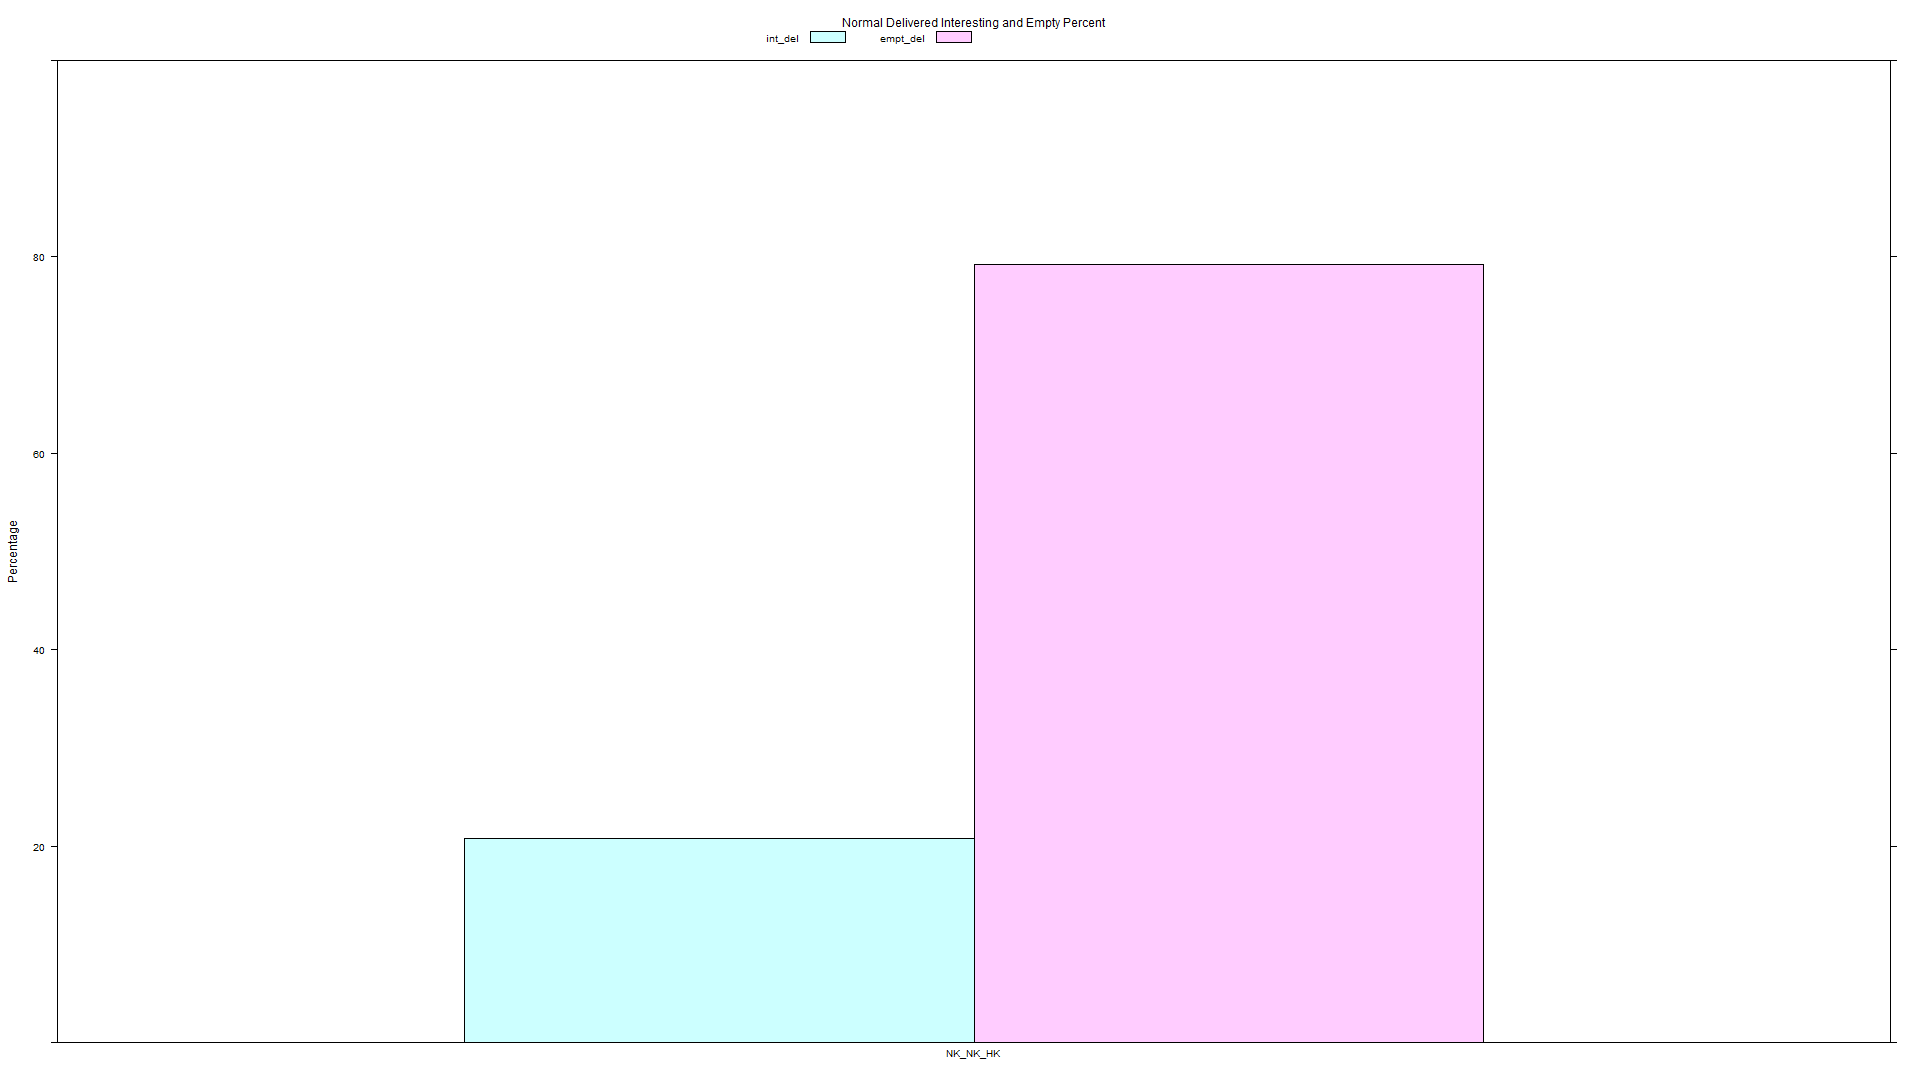
\includegraphics[width=0.8\textwidth]{Chap7/figures/plots/normal_ideal/emptvsint_percent_central.png}
% 	\caption{Interesting vs Empty Observations for Normal Saturation and Ideal Transmission Rate}
% 	\label{fig:sim:res:norm:ideal:emptint}
% 	\end{figure}

% 	\begin{figure}[H]
% 	\centering
% 	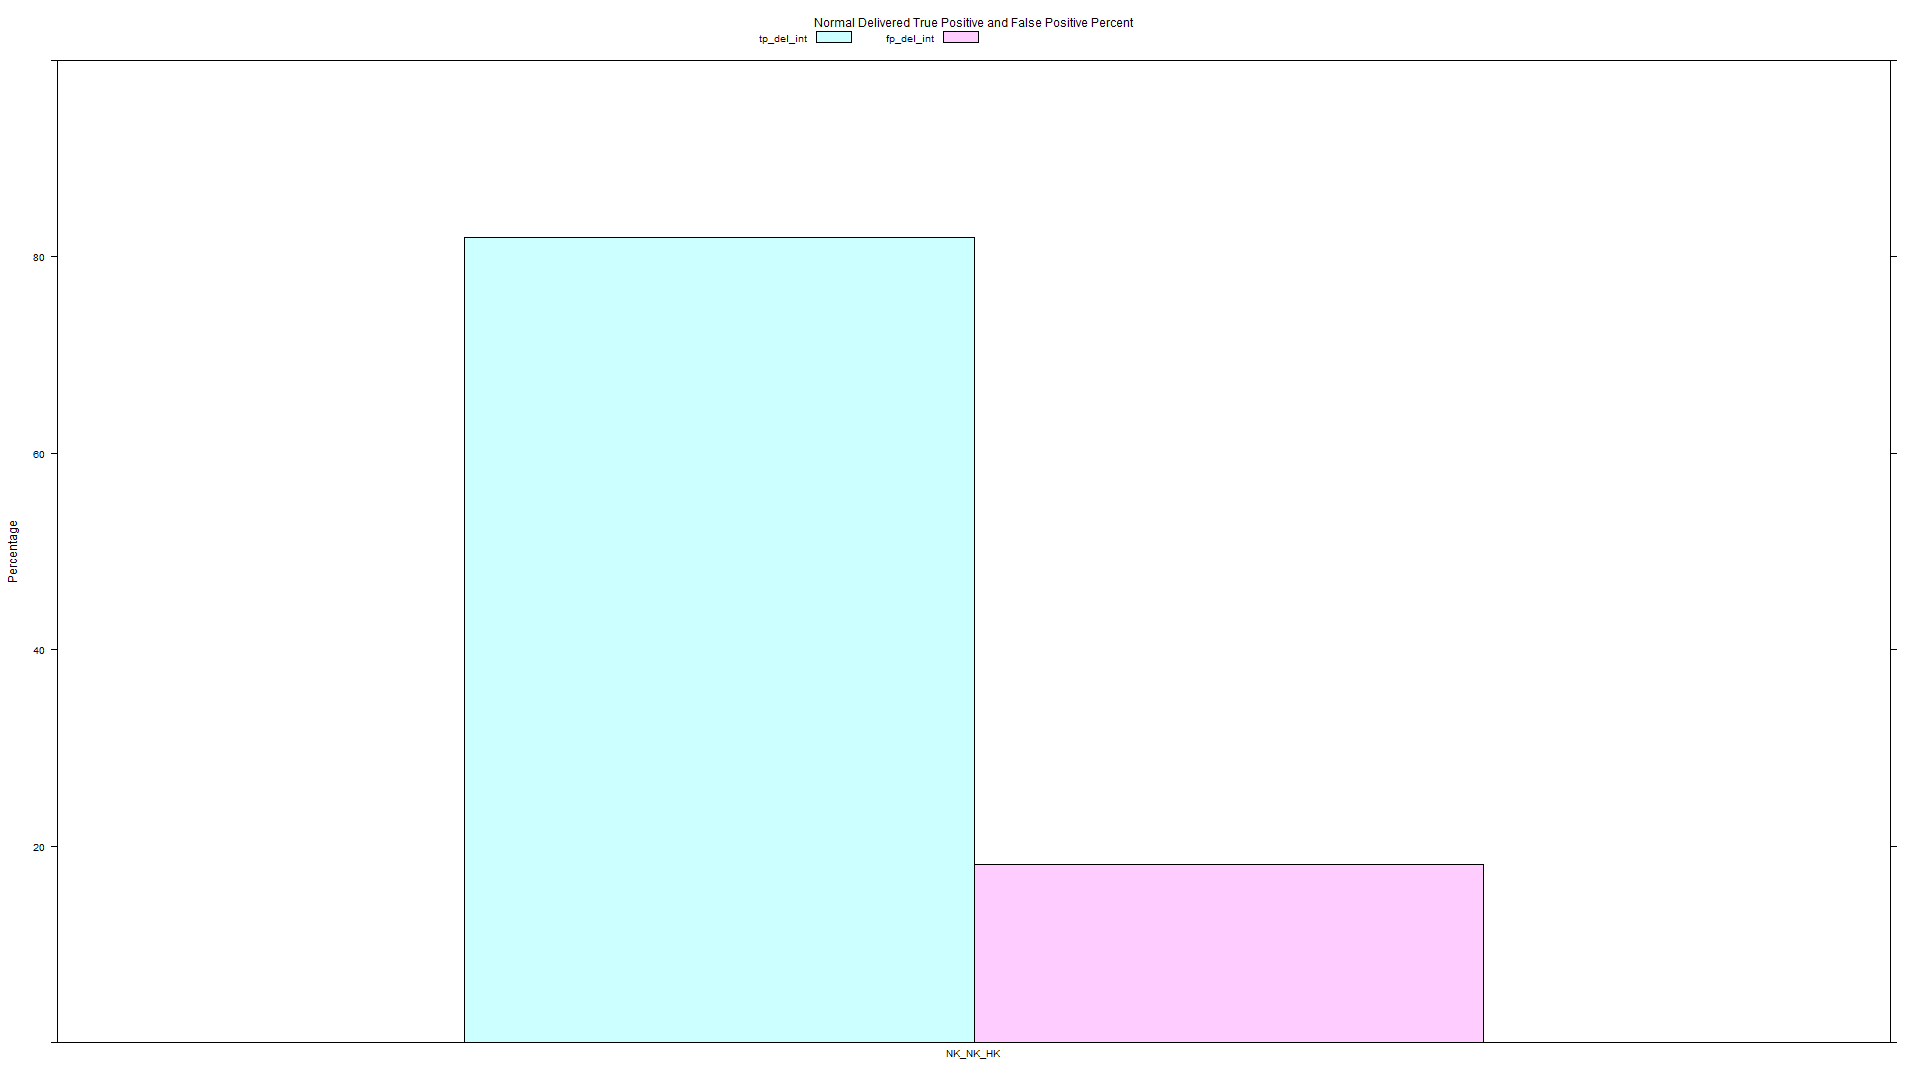
\includegraphics[width=0.8\textwidth]{Chap7/figures/plots/normal_ideal/tpvsfp_percent_central.png}
% 	\caption{TP vs FP Observations for Normal Saturation and Ideal Transmission Rate}
% 	\label{fig:sim:res:norm:ideal:tpfp}
% 	\end{figure}

% 	\begin{figure}[H]
% 	\centering
% 	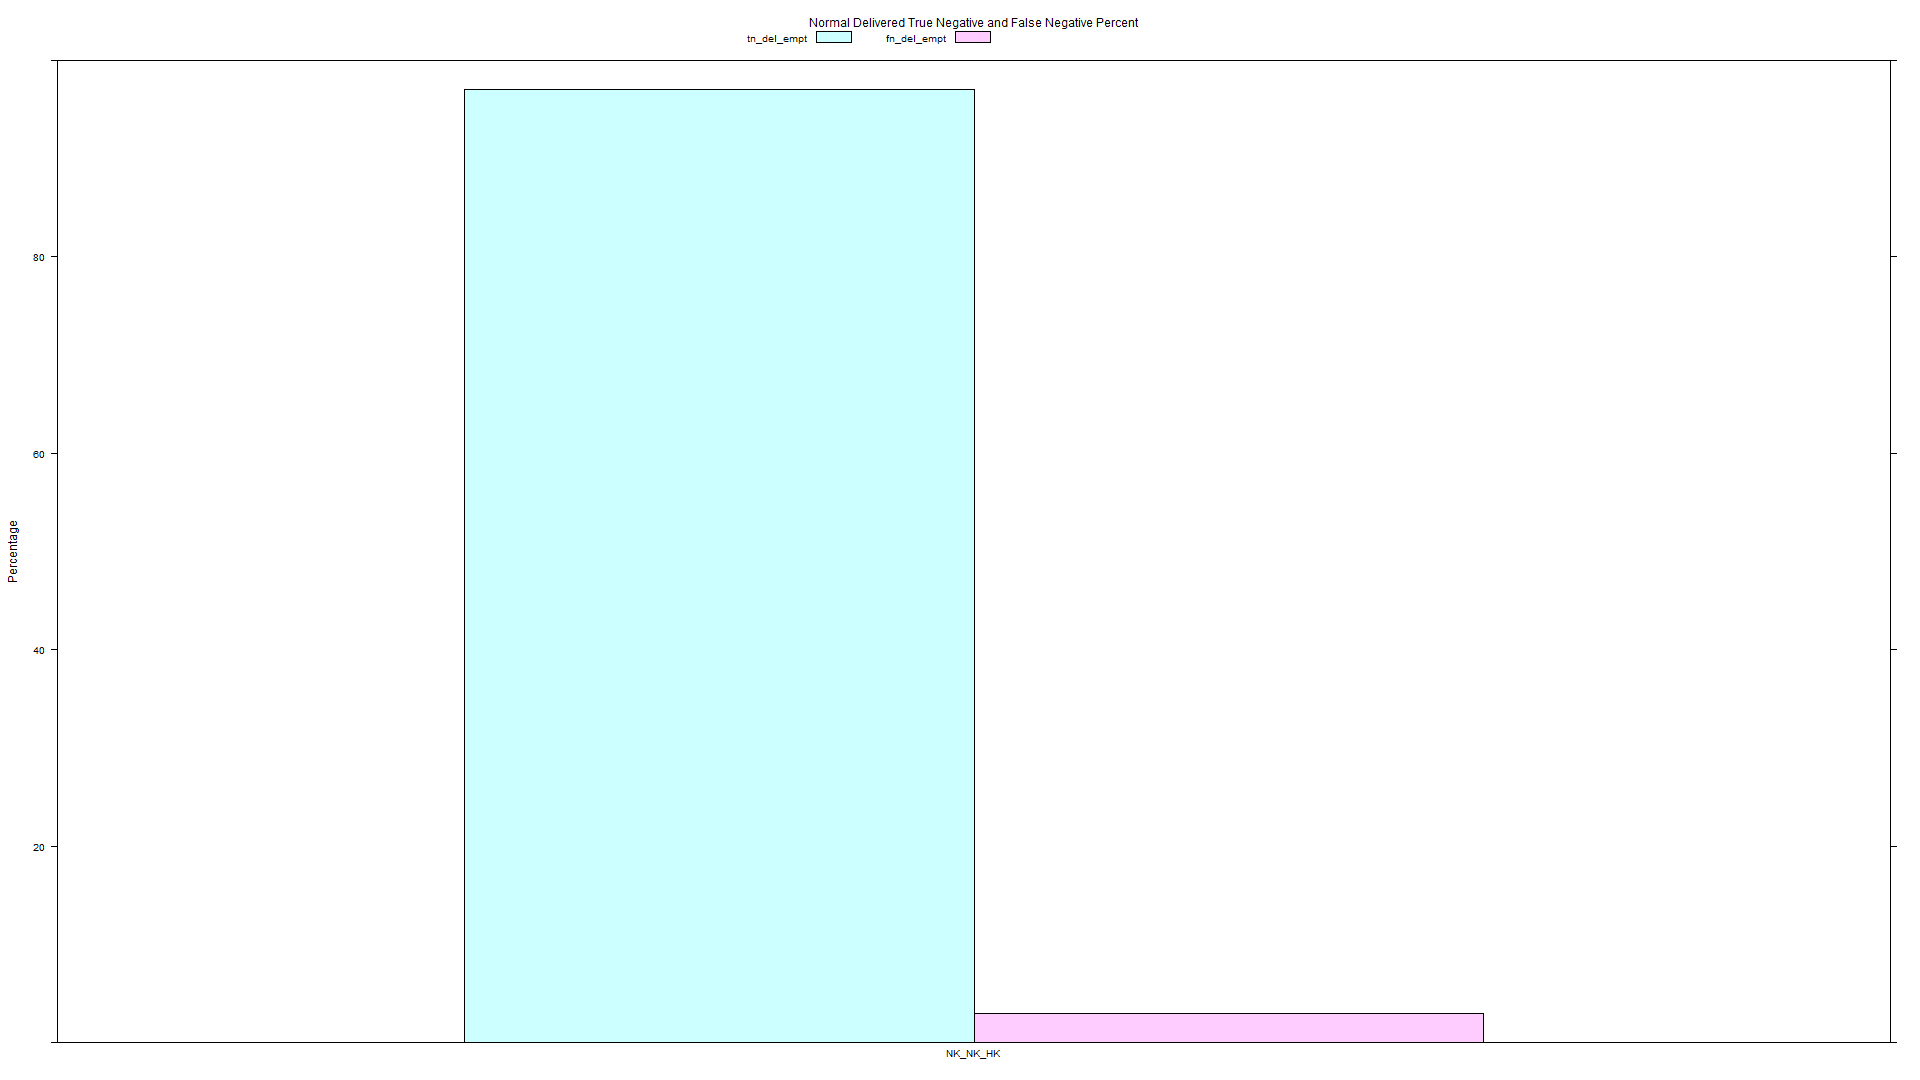
\includegraphics[width=0.8\textwidth]{Chap7/figures/plots/normal_ideal/tnvsfn_percent_central.png}
% 	\caption{FN vs FP Observations for Normal Saturation and Ideal Transmission Rate}
% 	\label{fig:sim:res:norm:ideal:tnfn}
% 	\end{figure}


% \subsubsection{Normal Bandwidth and Variable Transmission Rate}
% 	\begin{figure}[H]
% 	\centering
% 	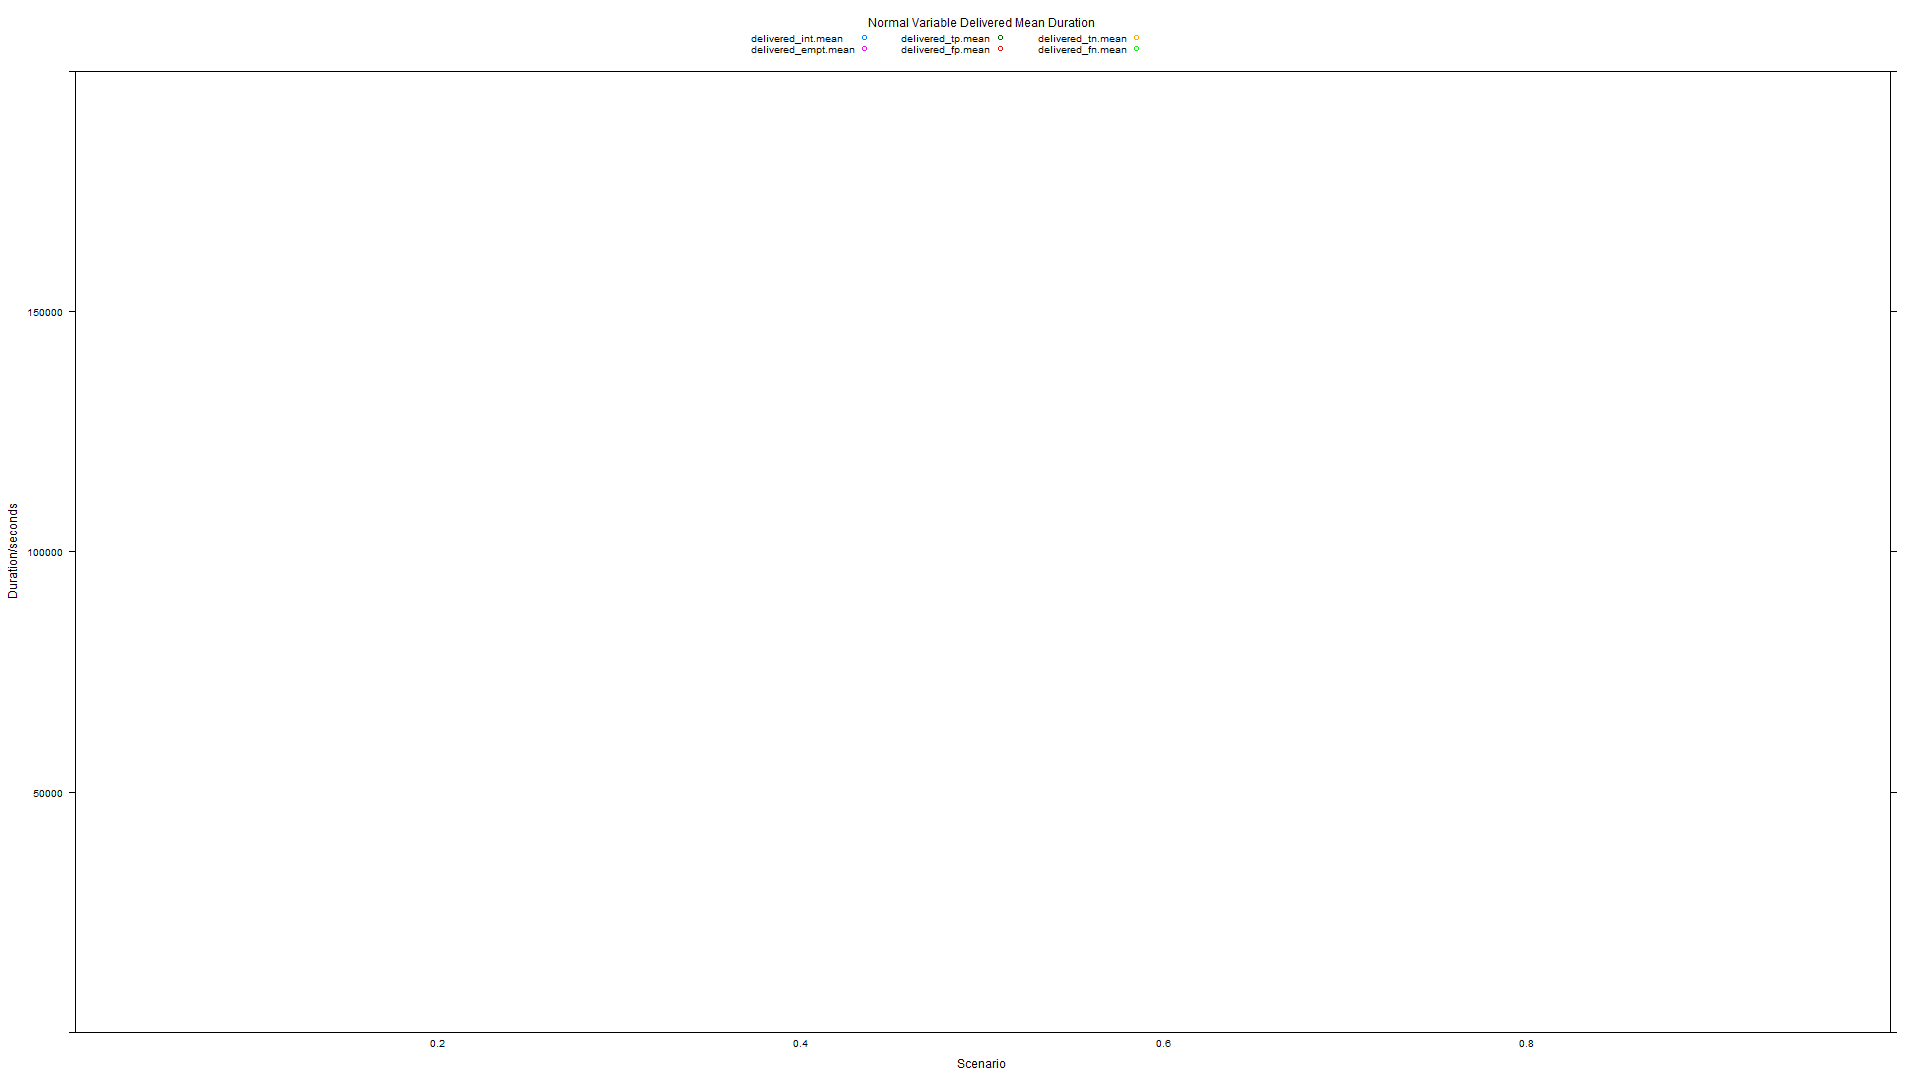
\includegraphics[width=0.8\textwidth]{Chap7/figures/plots/normal_variable/delivered_mean_central.png}
% 	\caption{Delivered Observations Mean Transmission Time for Normal Saturation and Variable Transmission Rate}
% 	\label{fig:sim:res:norm:variable:delmean}
% 	\end{figure}

% 	\begin{figure}[H]
% 	\centering
% 	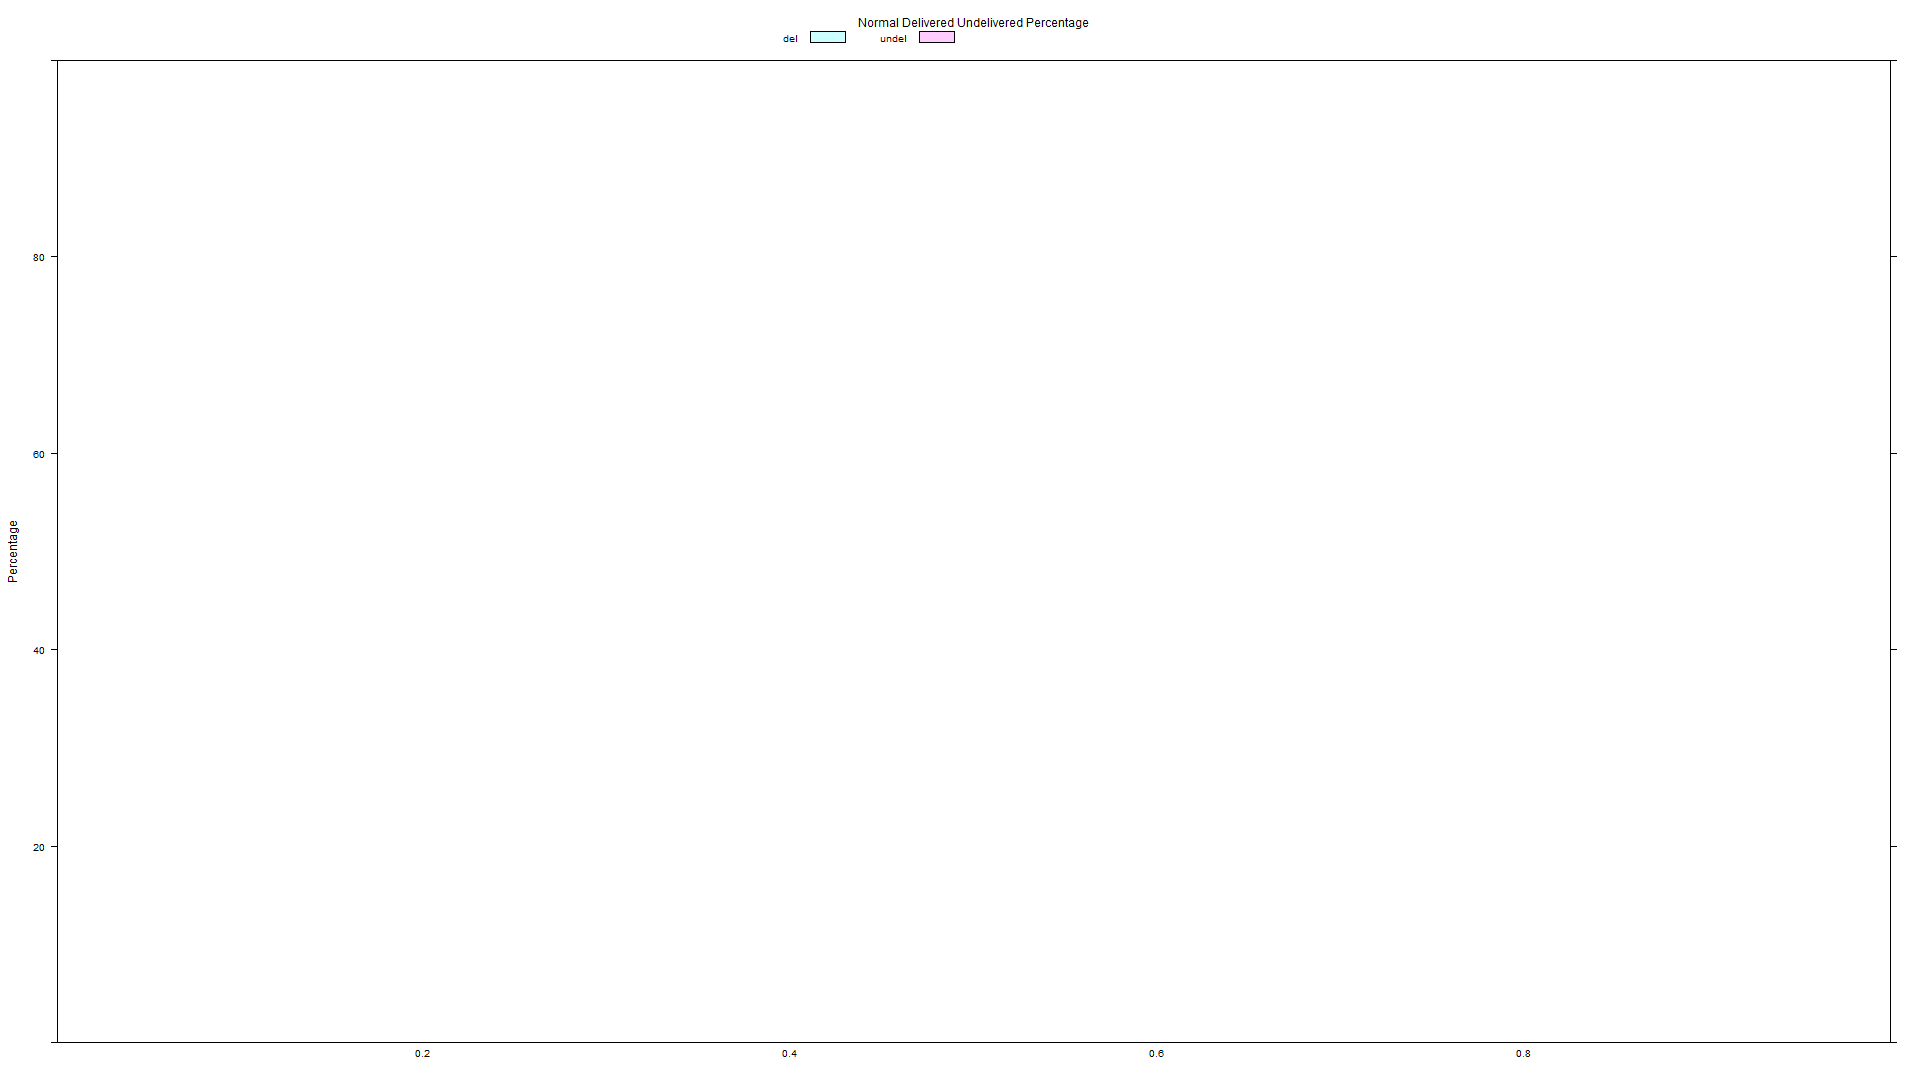
\includegraphics[width=0.8\textwidth]{Chap7/figures/plots/normal_variable/delvsundel_percent_central.png}
% 	\caption{Delivered vs Undelivered Observations for Normal Saturation and Variable Transmission Rate}
% 	\label{fig:sim:res:norm:variable:delundel}
% 	\end{figure}

% 	\begin{figure}[H]
% 	\centering
% 	
\includegraphics[width=0.8\textwidth]{Chap7/figures/plots/normal_variable/emptvsint_percent_central.png}
% 	\caption{Interesting vs Empty Observations for Normal Saturation and Variable Transmission Rate}
% 	\label{fig:sim:res:norm:variable:emptint}
% 	\end{figure}

% 	\begin{figure}[H]
% 	\centering
% 	
\includegraphics[width=0.8\textwidth]{Chap7/figures/plots/normal_variable/tpvsfp_percent_central.png}
% 	\caption{TP vs FP Observations for Normal Saturation and Variable Transmission Rate}
% 	\label{fig:sim:res:norm:variable:tpfp}
% 	\end{figure}

% 	\begin{figure}[H]
% 	\centering
% 	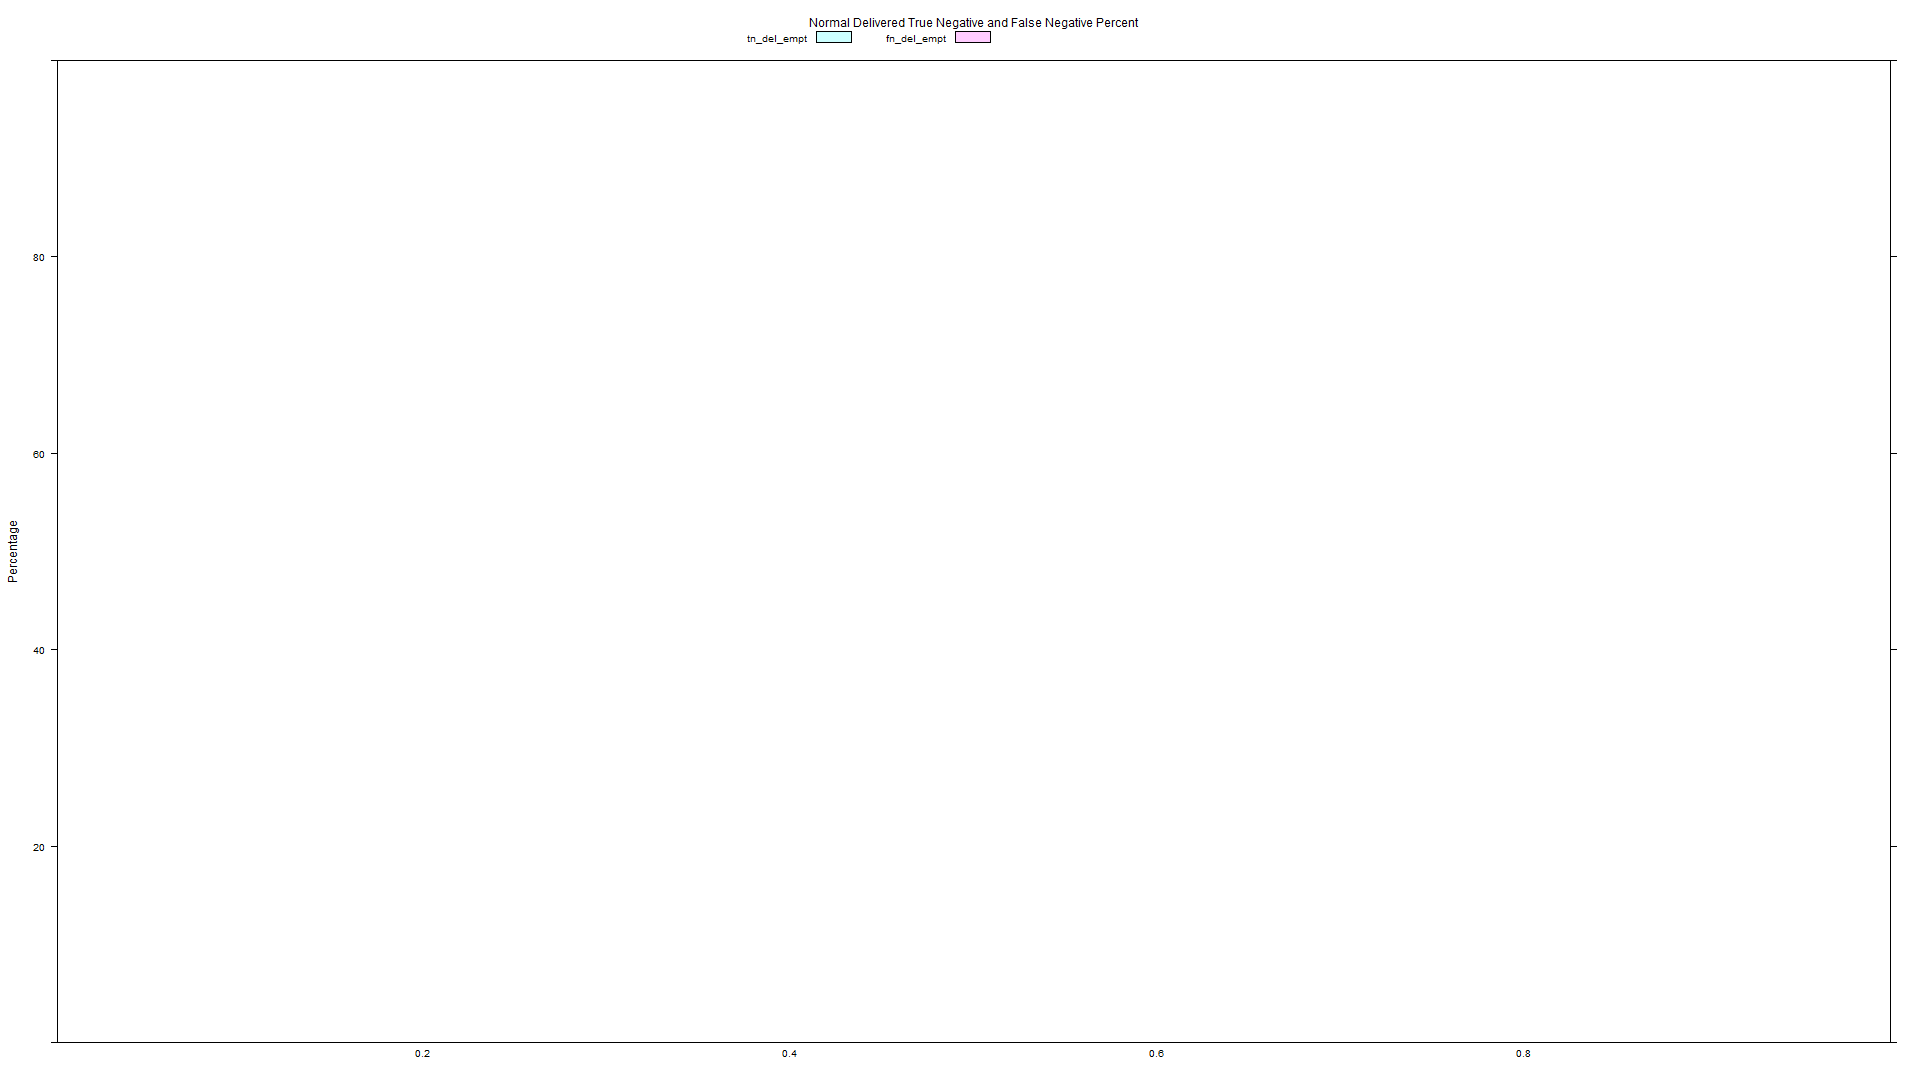
\includegraphics[width=0.8\textwidth]{Chap7/figures/plots/normal_variable/tnvsfn_percent_central.png}
% 	\caption{TN vs FN Observations for Normal Saturation and Variable Transmission Rate}
% 	\label{fig:sim:res:norm:variable:tnfn}
% 	\end{figure}

% \subsubsection{Saturated Bandwidth and Ideal Transmission Rate}
% 	\begin{figure}[H]
% 	\centering
% 	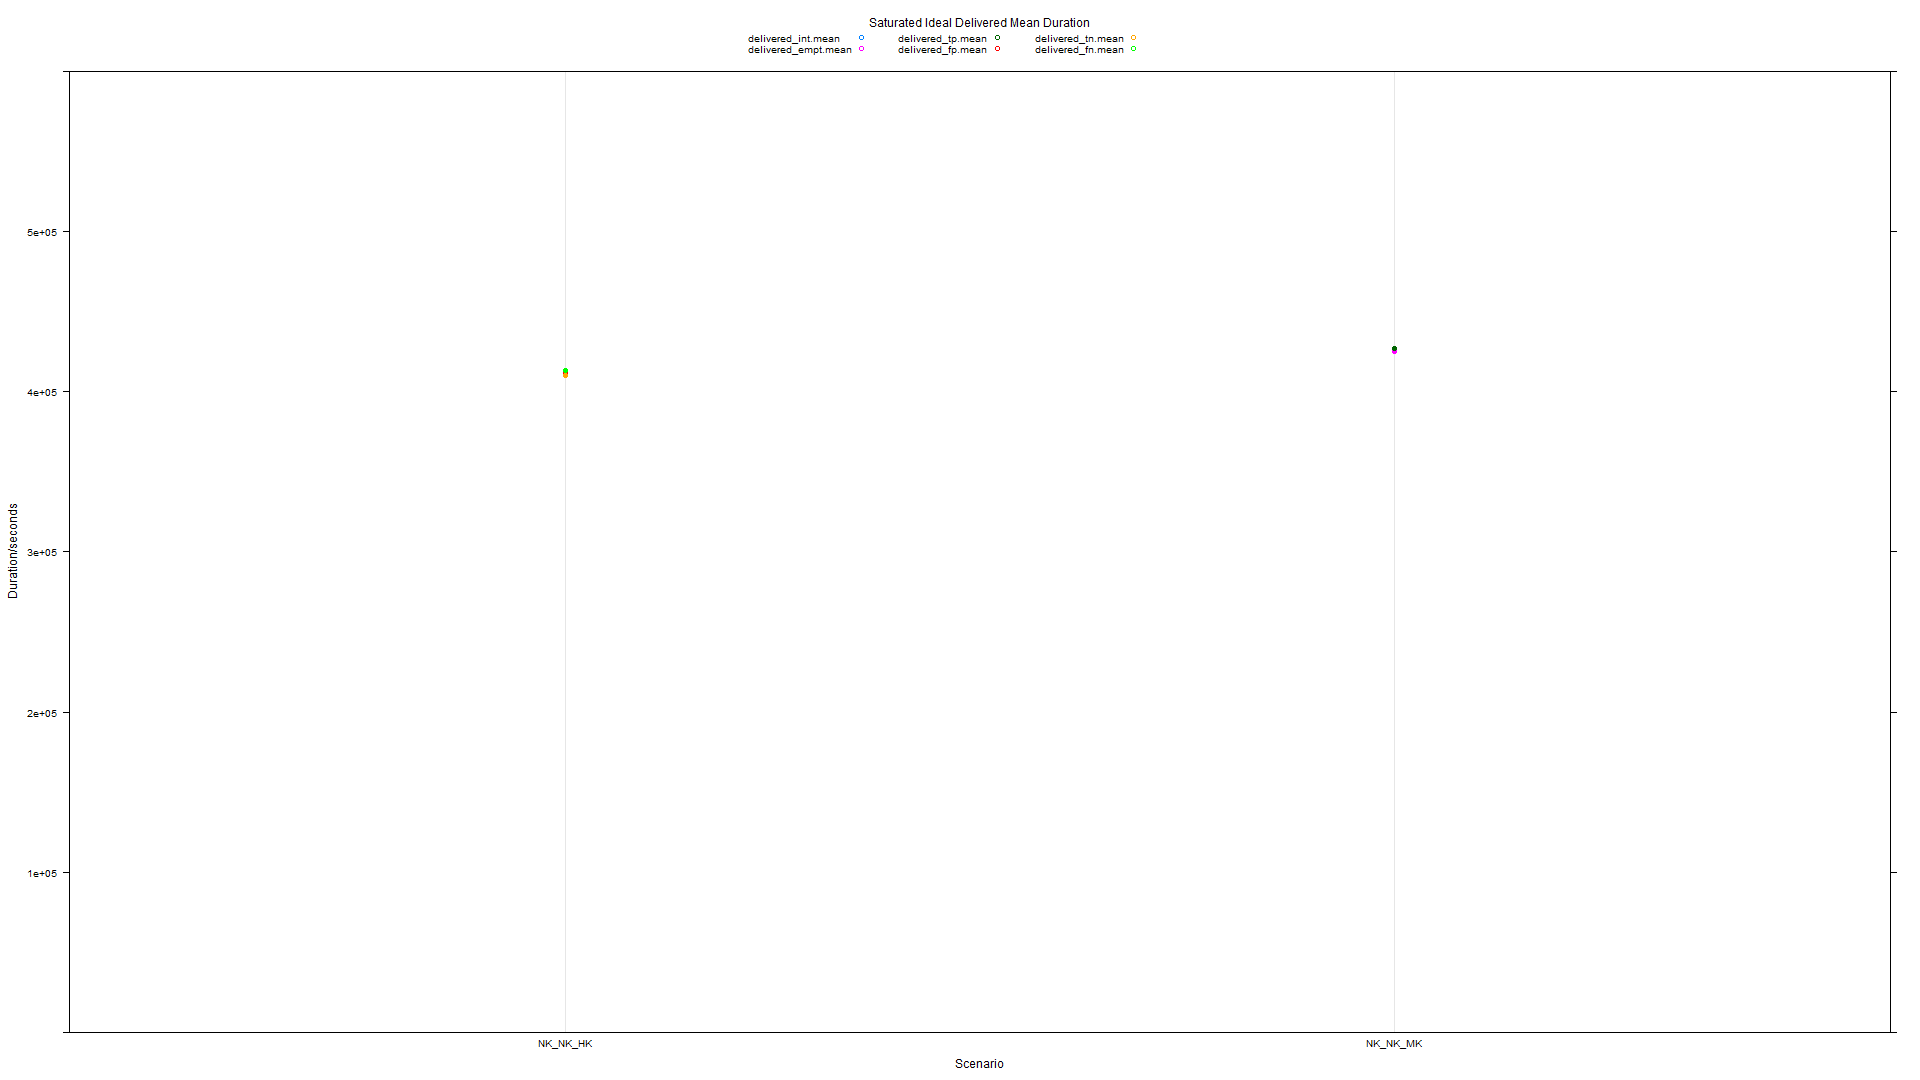
\includegraphics[width=0.8\textwidth]{Chap7/figures/plots/saturated_ideal/delivered_mean_central.png}
% 	\caption{Delivered Observations Mean Transmission Time for saturated Saturation and Ideal Transmission Rate}
% 	\label{fig:sim:res:sat:ideal:delmean}
% 	\end{figure}

% 	\begin{figure}[H]
% 	\centering
% 	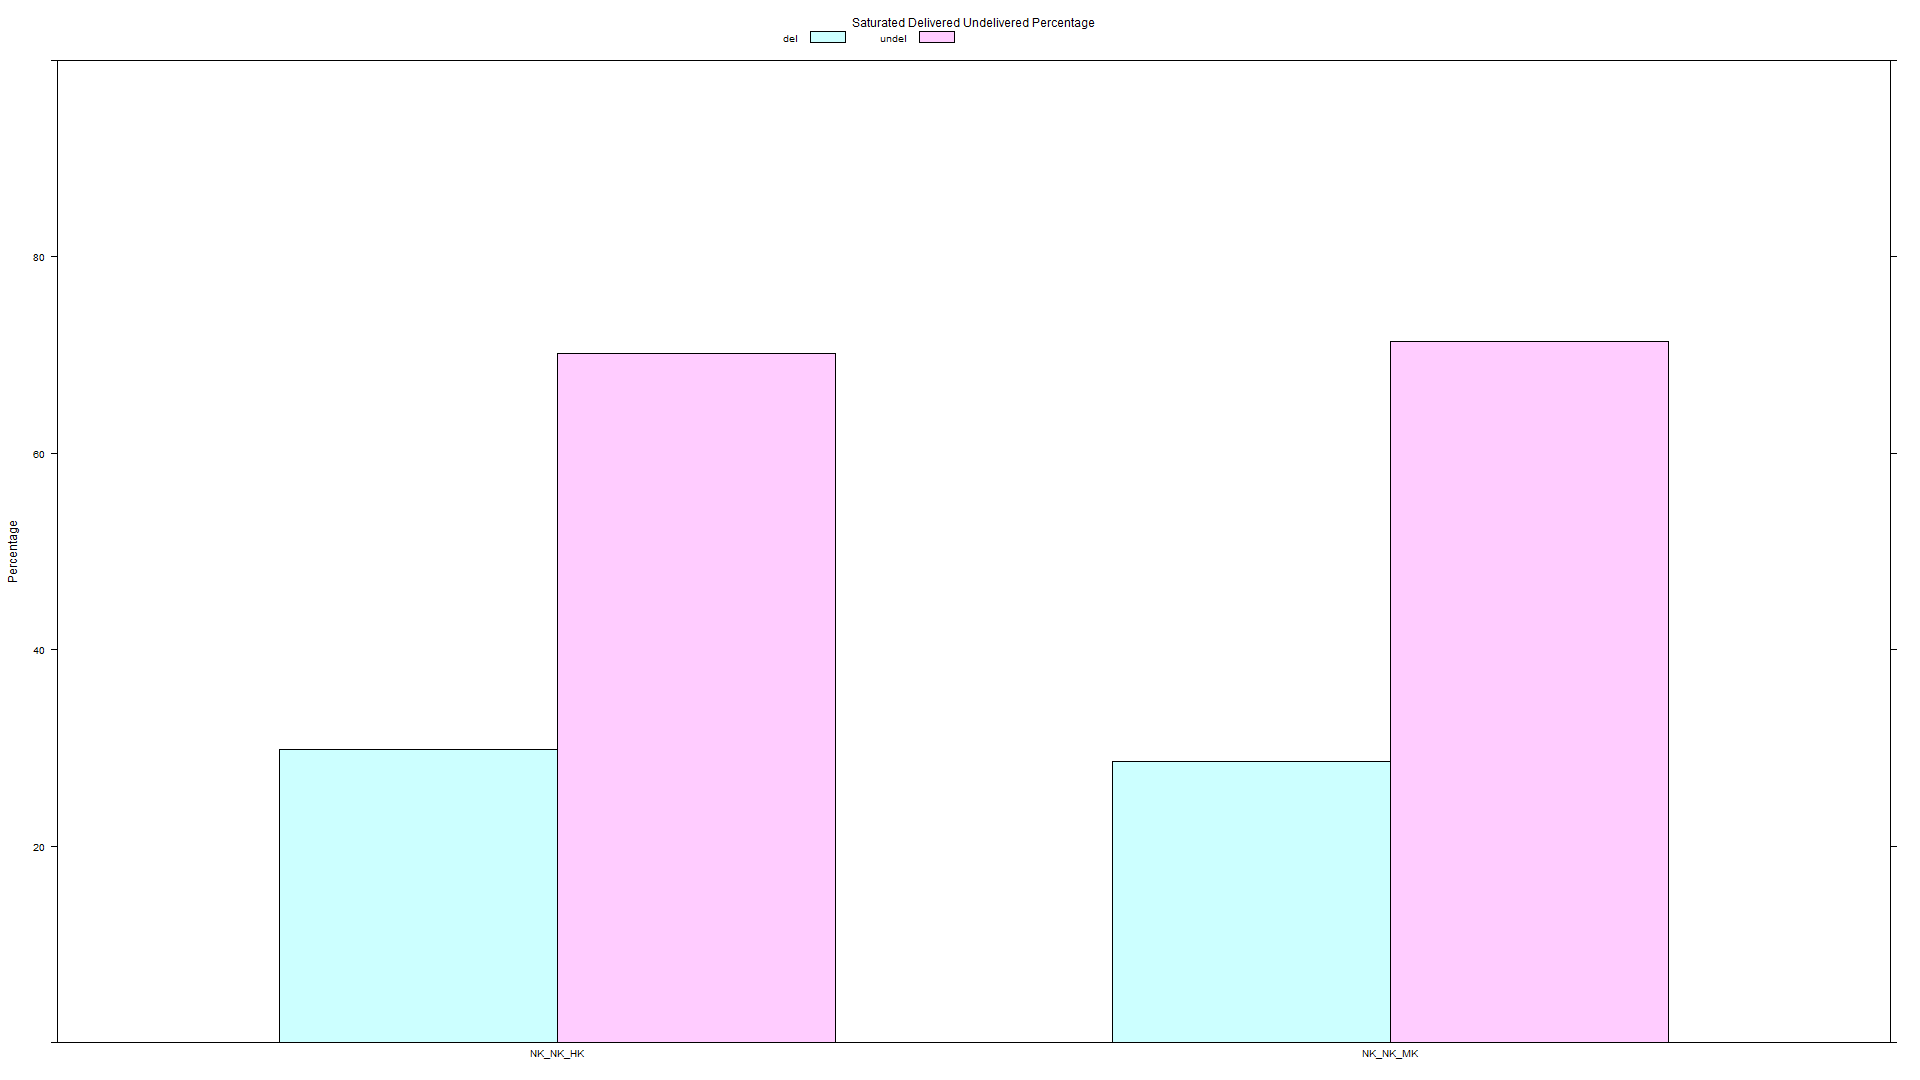
\includegraphics[width=0.8\textwidth]{Chap7/figures/plots/saturated_ideal/delvsundel_percent_central.png}
% 	\caption{Delivered vs Undelivered Observations for saturated Saturation and Ideal Transmission Rate}
% 	\label{fig:sim:res:sat:ideal:delundel}
% 	\end{figure}

% 	\begin{figure}[H]
% 	\centering
% 	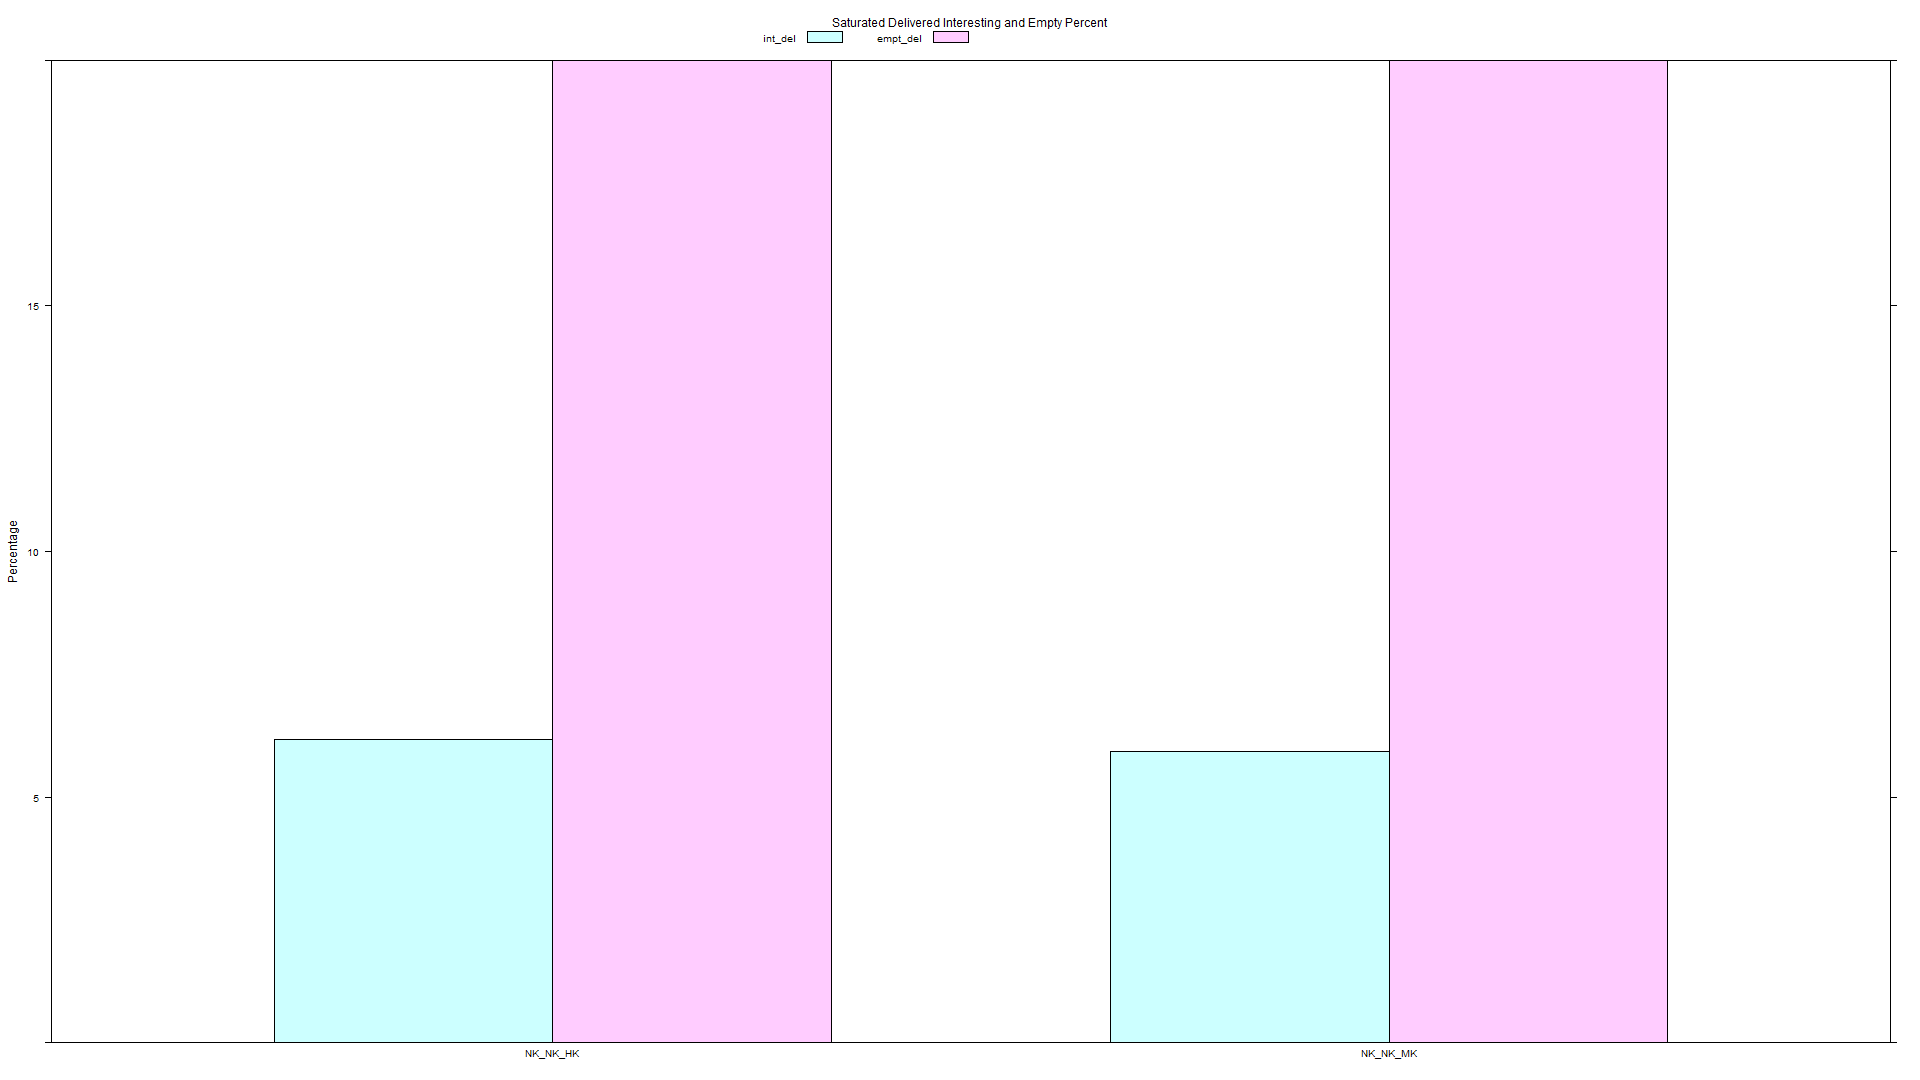
\includegraphics[width=0.8\textwidth]{Chap7/figures/plots/saturated_ideal/emptvsint_percent_central.png}
% 	\caption{Interesting vs Empty Observations for saturated Saturation and Ideal Transmission Rate}
% 	\label{fig:sim:res:sat:ideal:emptint}
% 	\end{figure}

% 	\begin{figure}[H]
% 	\centering
% 	
\includegraphics[width=0.8\textwidth]{Chap7/figures/plots/saturated_ideal/tpvsfp_percent_central.png}
% 	\caption{TP vs FP Observations for saturated Saturation and Ideal Transmission Rate}
% 	\label{fig:sim:res:sat:ideal:tpfp}
% 	\end{figure}

% 	\begin{figure}[H]
% 	\centering
% 	
\includegraphics[width=0.8\textwidth]{Chap7/figures/plots/saturated_ideal/tnvsfn_percent_central.png}
% 	\caption{TN vs FN Observations for saturated Saturation and Ideal Transmission Rate}
% 	\label{fig:sim:res:sat:ideal:tnfn}
% 	\end{figure}
	
% \subsubsection{Saturated Bandwidth and Variable Transmission Rate}
% 	\begin{figure}[H]
% 	\centering
% 	
\includegraphics[width=0.8\textwidth]{Chap7/figures/plots/saturated_variable/delivered_mean_central.png}
% 	\caption{Delivered Observations Mean Transmission Time for saturated Saturation and Variable Transmission Rate}
% 	\label{fig:sim:res:sat:variable:delmean}
% 	\end{figure}

% 	\begin{figure}[H]
% 	\centering
% 	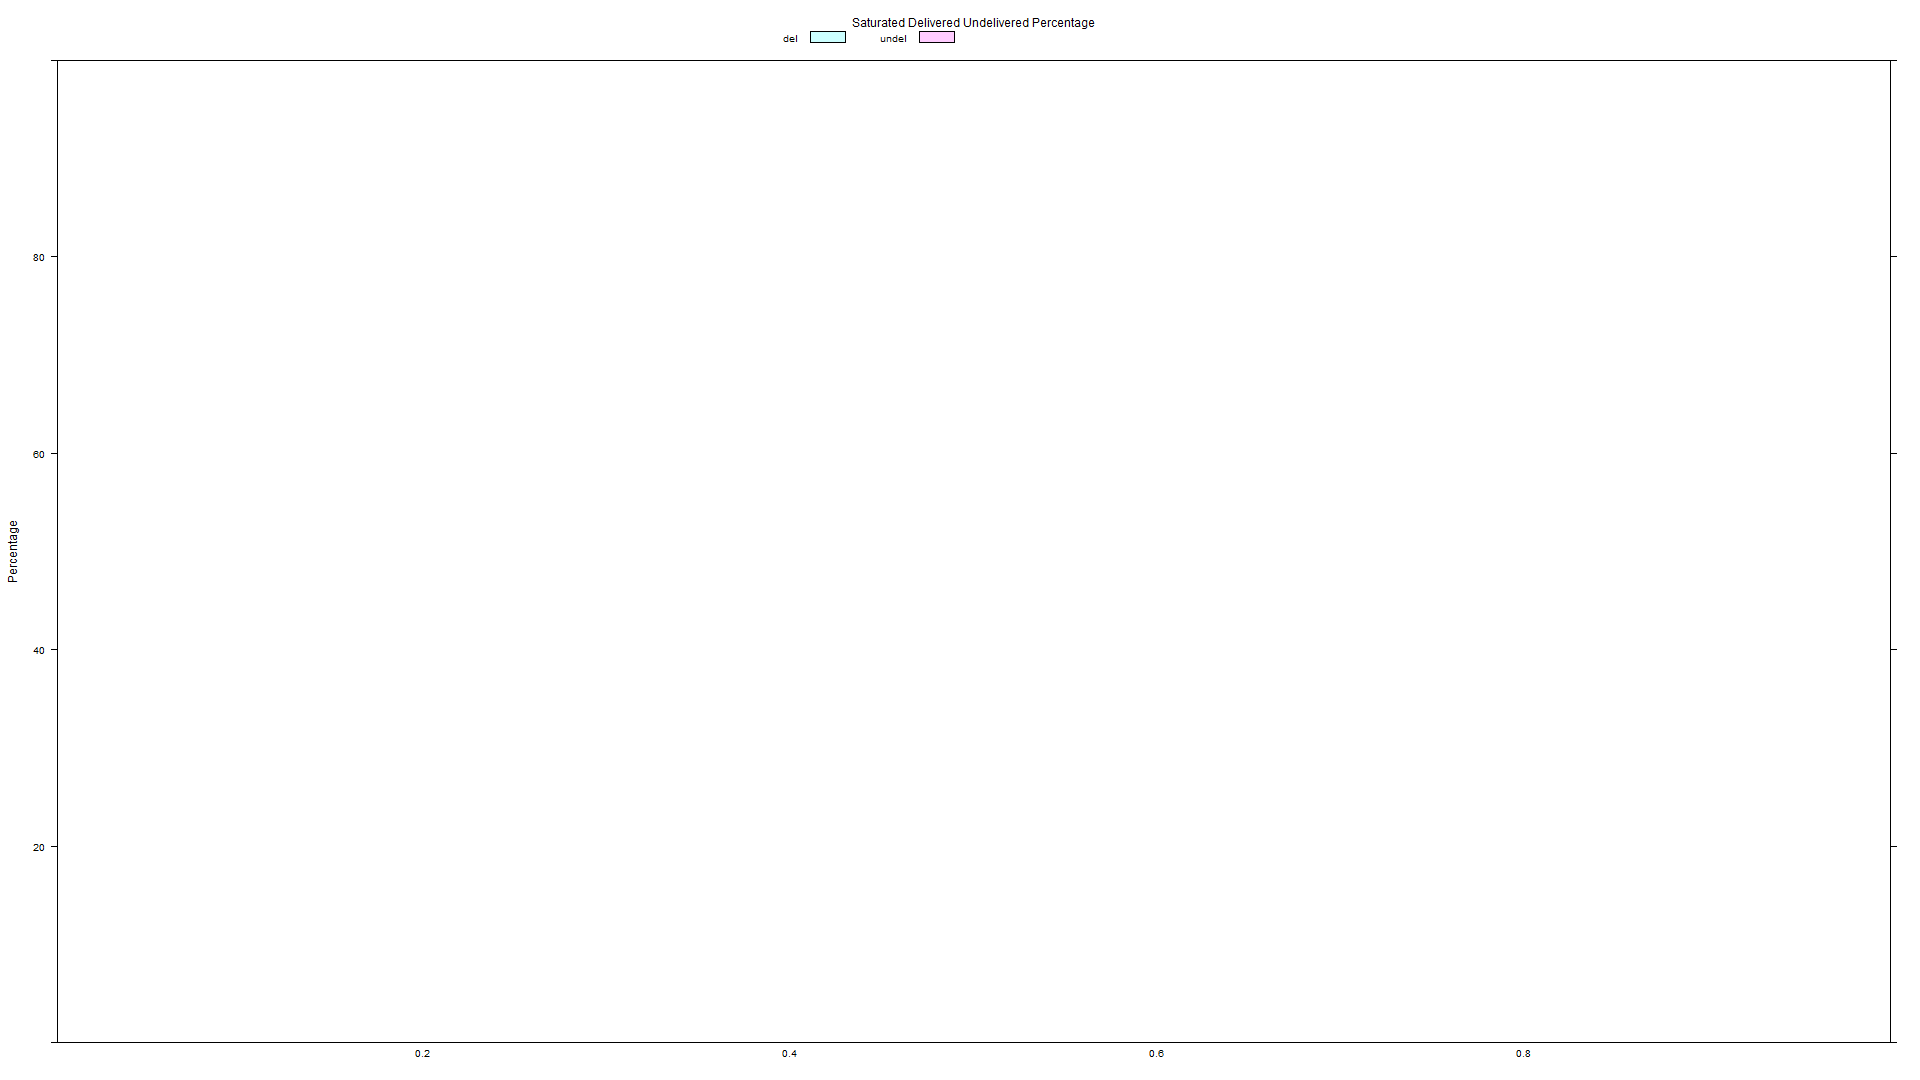
\includegraphics[width=0.8\textwidth]{Chap7/figures/plots/saturated_variable/delvsundel_percent_central.png}
% 	\caption{Delivered vs Undelivered Observations for saturated Saturation and Variable Transmission Rate}
% 	\label{fig:sim:res:sat:variable:delundel}
% 	\end{figure}

% 	\begin{figure}[H]
% 	\centering
% 	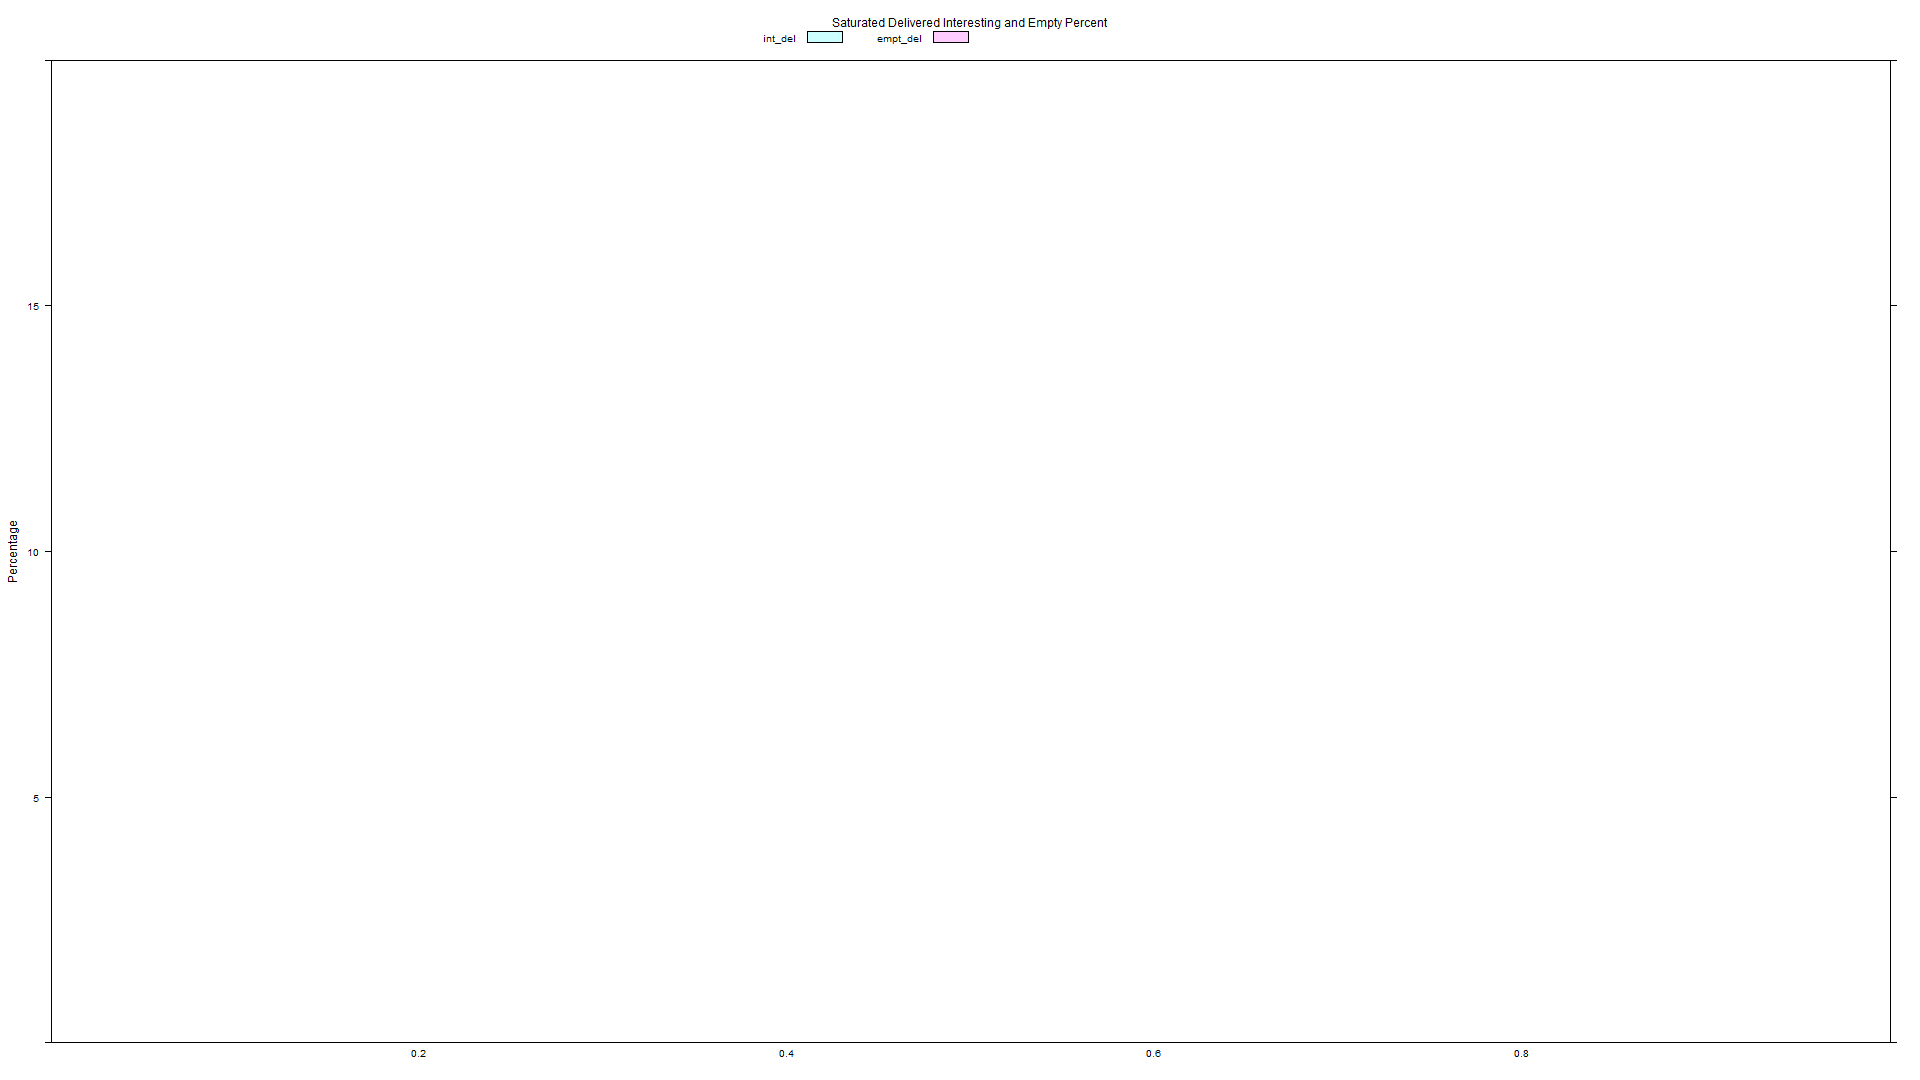
\includegraphics[width=0.8\textwidth]{Chap7/figures/plots/saturated_variable/emptvsint_percent_central.png}
% 	\caption{Interesting vs Empty Observations for saturated Saturation and Variable Transmission Rate}
% 	\label{fig:sim:res:sat:variable:emptint}
% 	\end{figure}

% 	\begin{figure}[H]
% 	\centering
% 	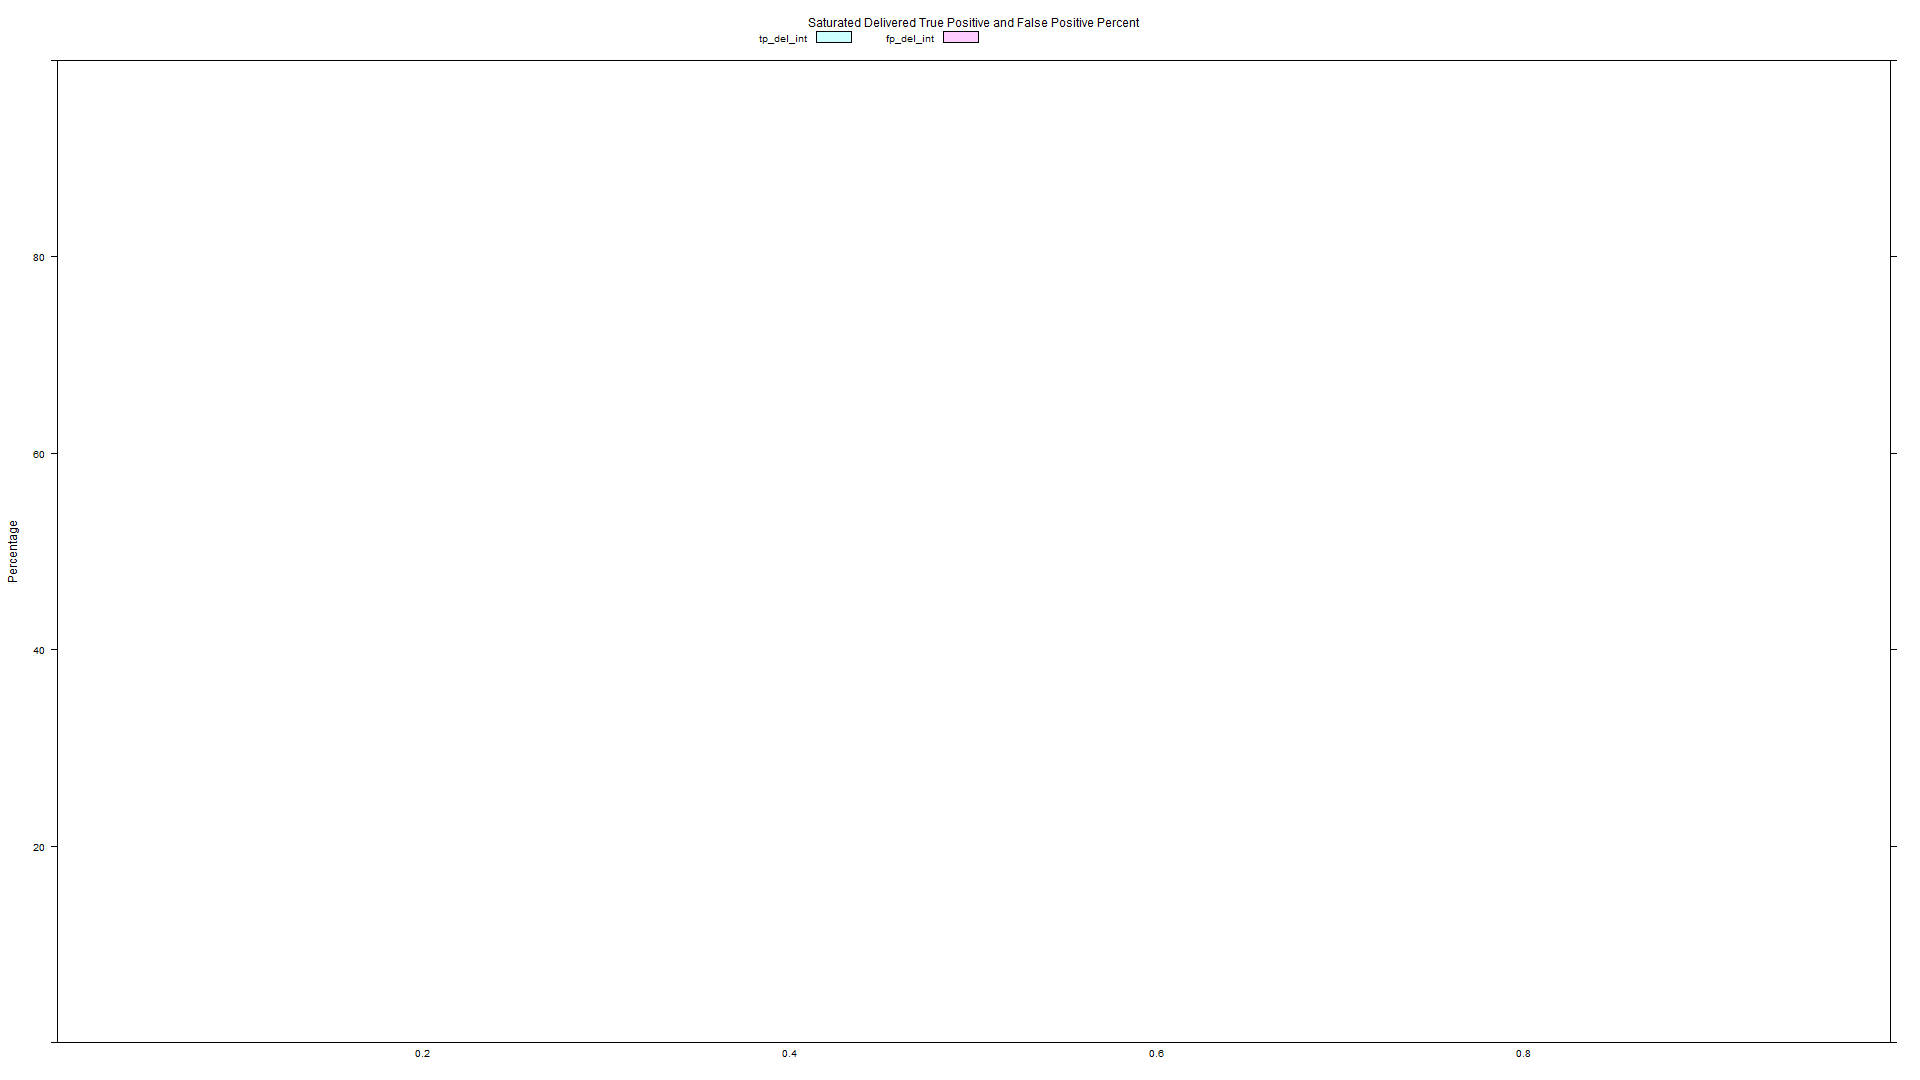
\includegraphics[width=0.8\textwidth]{Chap7/figures/plots/saturated_variable/tpvsfp_percent_central.png}
% 	\caption{TP vs FP Observations for Saturated Saturation and Variable Transmission Rate}
% 	\label{fig:sim:res:sat:variable:tpfp}
% 	\end{figure}

% 	\begin{figure}[H]
% 	\centering
% 	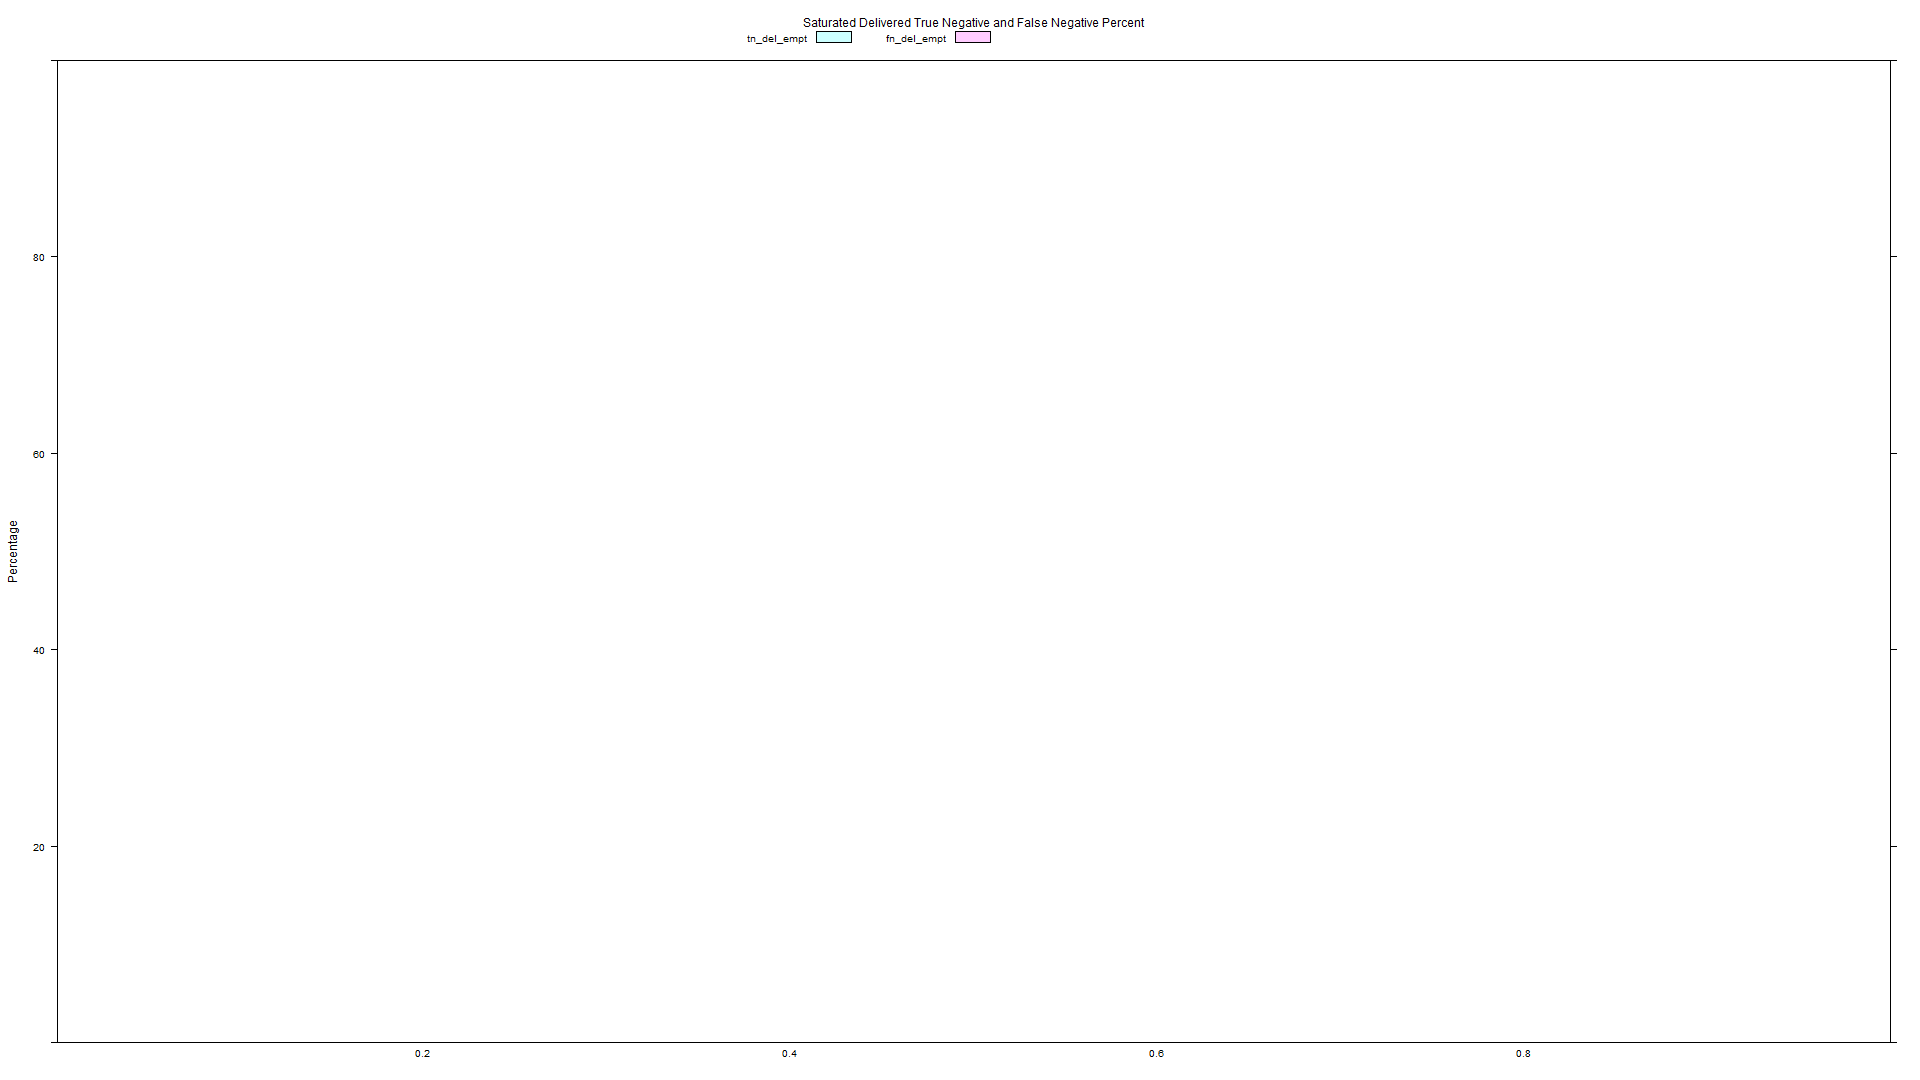
\includegraphics[width=0.8\textwidth]{Chap7/figures/plots/saturated_variable/tnvsfn_percent_central.png}
% 	\caption{TN vs FN Observations for Saturated Saturation and Variable Transmission Rate}
% 	\label{fig:sim:res:sat:variable:tnfn}
% 	\end{figure}



































